\documentclass[12pt]{report}
\usepackage{amsfonts}
\usepackage{amsmath}
\usepackage[hidelinks]{hyperref}
\usepackage[spanish, es-nodecimaldot]{babel}
\usepackage[utf8]{inputenc}
\usepackage{geometry}
\usepackage{graphicx}
\usepackage{hyphenat}
\usepackage{listings}
\usepackage{minted}
\usepackage{multirow}
\usepackage{relsize}
\usepackage{xcolor}

\graphicspath{{img/}}

\newgeometry{
	right=3cm,
	left=3cm,
	top=2.5cm,
	bottom=2.5cm
}

\hypersetup{
	colorlinks,
	citecolor=black,
	filecolor=black,
	linkcolor=black,
	urlcolor=black
}

% Profundidad de secciones
\setcounter{tocdepth}{4}
\setcounter{secnumdepth}{4}

% Referencias automáticas
\def\sectionautorefname{sección}
\def\subsectionautorefname{subsección}
\def\subsubsectionautorefname{subsección}

% Índice
\addto\captionsspanish{
	\renewcommand{\contentsname}%
	{Índice}%
}

\begin{titlepage}

\title{
	\begin{figure}
		\centering
			\includegraphics[width=2cm, height=3cm]{img/logo.png}\\
			{Universidad del Bío-Bío\\
			Facultad de Ciencias Empresariales\\
			Depto. de Sistemas de Información}
	\end{figure}
	{Desarrollo de una aplicación web para la comunidad de Re-Volt America}\\
	{\large Proyecto de título para optar al título de Ingeniero de Ejecución en Computación e Informática}
}
\author{José Benavente}
\date{Lunes 18 de diciembre, 2023}

\end{titlepage}

\begin{document}

\maketitle

\tableofcontents

\chapter*{Abstracto}
\addcontentsline{toc}{section}{Abstracto}
\input{chapters/abstract.tex}

\chapter*{Dedicatoria}
\addcontentsline{toc}{section}{Dedicatoria}
El presente proyecto está dedicado a toda la comunidad de Re-Volt, en especial a quienes forman parte del grupo de jugadores de Re-Volt America.

Sin lugar a dudas, durante los últimos años, este juego pasó de ser un simple pasatiempo a convertirse en algo muy importante para mí a nivel personal. Muchas de las personas que he conocido a través de Re-Volt se han convertido, ya a estas alturas, en buenos amigos a quienes valoro muchísimo. Todos han sabido siempre apreciar mi trabajo, y por eso les estoy infinitamente agradecido. Sin ustedes, nada de lo que amo hacer tendría trascendencia alguna. De todo corazón, muchas gracias. Es por todo lo anterior que no podría dedicar este trabajo a nadie si no a ustedes.


\chapter*{Agradecimientos}
\addcontentsline{toc}{section}{Agradecimientos}
En primer lugar, se extiende un agradecimiento formal a los siguientes desarrolladores quienes, de una forma u otra, han contribuido a la base de código del presente proyecto:
\begin{itemize}
	\item Marco Roth. Por ayudar con la migración del proyecto a ''esbuild'', y por resolver problemas con HAML.
	\item Nicolás Duque. Por probar la instalación del proyecto en plataformas de Linux, testear el proyecto en su fase beta, y por ayudar con la implementación de traducciones en la web.
\end{itemize}

También se les extiende un agradecimiento a todos quienes han hecho una donación voluntaria, sin importar el monto que fuese, al desarrollador principal de este proyecto a través de GitHub Sponsors durante el desarrollo de esta tesis:
\begin{itemize}
	\item Vicente Aguilera.
	\item Gabriel Carnielli.
	\item Dario Chaile.
	\item Benjamín Contreras.
	\item Benjamín Ferrada.
	\item Josafat jiménez.
	\item  Mateusz Kobylański.
	\item Jorge Matamala.
	\item Benjamín Mosso.
	\item Leandro Rodríguez.
	\item Juan Pablo Rosas.
\end{itemize}


\chapter*{Resumen}
\addcontentsline{toc}{section}{Resumen}
VENDER REVOLT AMERICA:

RV AMERICA HA QUEDADO ATRAS EN CUANTO A SU SOPORTE Y GRACIAS A ESTE PROYECTO CRECERÁ Y SE VOLVERÁ MÁS MASIVO ETC...


El presente informe trata de una aplicación que busca centralizar toda la información relacionada a las sesiones multijugador del videojuego Re-Volt celebradas por la comunidad de Re-Volt America, la cual busca mejorar la experiencia de usuario para los administradores encargados de mantener los registros de resultados y tablas de puntuación de Re-Volt America actualizadas, además de servir como un cambio revolucionario para todos aquellos que buscan conseguir una experiencia competitiva dentro del videojuego. 


\chapter*{Introducción}
\addcontentsline{toc}{section}{Introducción}
Dentro de las comunidades del videojuego de carreras Re-Volt, 1999, Re-Volt America se ha quedado atrás en lo que refiere a su sistema interno de cálculo de resultados y estadísticas por jugador. Esta problemática genera el surgimiento de este proyecto, el cual pretende modernizar y mejorar la gestión interna de Re-Volt America, así como también busca enriquecer la experiencia de usuario como nunca antes se ha visto en la escena de las comunidades de Re-Volt.

El presente informe trata de una aplicación que busca centralizar toda la información relacionada a las sesiones multijugador del videojuego Re-Volt celebradas por la comunidad de Re-Volt America, logrando así mejorar la experiencia de usuario para los administradores encargados de mantener los registros de resultados y tablas de puntuación, además de servir como un cambio revolucionario para todos aquellos que buscan conseguir una experiencia competitiva dentro del videojuego. 


% Estudio del Problema
\chapter{Estudio del Problema}

\section{Definiciones, Siglas y Abreviaciones}
A continuación, se definirán algunos conceptos relevantes en el contexto del videojuego Re-Volt y la comunidad de Re-Volt America:

\begin{itemize}
	\item Re-Volt: El videojuego Re-Volt, 1999 (https://en.wikipedia.org/wiki/Re-Volt).
	\item RV: Re-Volt.
	\item RVGL: Re-Volt: OpenGL. La reescritura del juego original que es usada por todos los jugadores hoy en día. (https://rvgl.org).
	\item Re-Volt I/O: Comunidad Europea de Re-Volt.
	\item RVA: Re-Volt America.
	\item Sesión: Evento de carreras online del videojuego Re-Volt, en donde dos o más personas compiten en dos o más carreras multijugador.
	\item Session Log: Archivo separado por comas que contiene un registro crudo de los resultados de las carreras jugadas en una sesión de RVGL.
\end{itemize}

\section{Historia de Re-Volt}
Re-Volt America, en su expresión más simple, es una comunidad de jugadores del videojuego Re-Volt, el cual fue lanzado originalmente en el año 1999 por Acclaim Studios en Londres. Re-Volt es un videojuego de carreras y simulador arcade de autos a control remoto, el cual explora una premisa en donde dichos autos compiten en carreras de radio control en ambientes como museos, supermercados, barcos, sitios de construcción, entre otros. Esto combinado con una mecánica de objetos que pueden ser recogidos por dichos autos para atacar a los competidores, obtener más velocidad, entre otras ventajas.

El arte original de la caratula del juego puede ser apreciado en la figura FIGNUM.

\includegraphics{img/re-volt.jpg}

El primero de septiembre del año 2004, Acclaim Studios se declara en banca rota, y cesa permanentemente todo el desarrollo y mantenimiento que en algún momento proveyó a Re-Volt y a su comunidad. Este suceso, a lo largo de los años, dio lugar a muchas comunidades segmentadas del juego en el internet de ese entonces. Con el tiempo, nuevos sitios y proyectos comenzaron a surgir, tales como el portal web de Re-Volt Race, una página de Re-Volt que se dedicaba a organizar partidas online y mantener tablas de resultados para los jugadores, o Re-Volt: OpenGL (RVGL), una re-escritura moderna del Re-Volt original que todos conocían, ahora disponible para plataformas modernas y otros sistemas operativos además de Windows, como Linux, MacOS, e incluso una versión para dispositivos Android.

Dentro de lo anteriormente enmarcado, aparece en el año 2015 la comunidad de Re-Volt I/O, cuyo logotipo se puede apreciar en la figura FIGNUM. Esta comunidad estaba formada por un grupo de jugadores de Re-Volt, principalmente europeos, quienes incursionaron por primera vez en intentar crear una plataforma estable para el videojuego y su comunidad de jugadores. Este sería un lugar en donde cualquiera que quisiera disfrutar del juego podría encontrar guías de ayuda, tutoriales, descargas y demás contenido para poder instalar y jugar Re-Volt en su computador o dispositivo móvil.

\includegraphics{img/io.png}

En sus inicios, Re-Volt I/O adoptó a RVGL como la distribución estándar de Re-Volt que ofrecería a sus jugadores, haciéndole ganar público y reconocimiento al proyecto publicando enlaces de descarga directos en su página web (re-volt.io), además de entregar soporte y mantener hilos de discusión relacionados con RVGL y sus actualizaciones en su foro oficial (forum.re-volt.io).

En adición a lo anterior, RVGL no era tan sólo una versión modernizada del Re-Volt original, sino que también traía consigo el aspecto más importante que tiene Re-Volt en la actualidad, y el cual mantiene unida y activa a su comunidad en general: el modo multijugador u online. Dicho modo no sólo permitía a los jugadores correr carreras en línea, sino que, además, extendía soporte para que miembros de la comunidad pudiesen diseñar sus propios autos y pistas de manera personalizada, agrandando así, de manera casi infinita, el repertorio de contenido descargable para Re-Volt.

Re-Volt I/O adoptó un sistema en donde su administración elige ciertos autos y pistas hechos por la comunidad cada ciertos meses. De esta forma, todos estos autos y pistas, elegidos a votación, terminan juntos en un paquete de contenido de extensión para RVGL, el cual Re-Volt I/O se encarga de distribuir para que sus usuarios lo descarguen y puedan jugar en línea. De manera habitual, tener este paquete de contenido es obligatorio para poder jugar en las sesiones multijugador organizadas por Re-Volt I/O, lo cual lo convertiría en un estándar para los jugadores que quisieran incorporarse a la comunidad en toda su extensión.

Fue así como Re-Volt I/O, entre finales del 2015 y mediados del 2017, logró consolidarse y llegar a más jugadores que nunca, formando una comunidad activa de amantes del juego quienes, espontáneamente, se reunían a jugar en línea durante la semana utilizando un paquete de contenido adicional para RVGL, el cual todos debían descargar e instalar por separado para poder jugar. Eventualmente, estas partidas en línea adquirieron un horario definido con fechas y horas acordadas con antelación, para así facilitar la asistencia de los jugadores a los eventos de carreras.

En la actualidad, Re-Volt I/O sigue siendo la comunidad de Re-Volt más grande en términos de jugadores y escala, pero en si todas las comunidades de Re-Volt están unidas y se ayudan unas con otras. Después de todo, se trata de un juego nicho, en donde todos intentan hacerlo accesible y fácil de entender para quienes deseen formar parte de su comunidad.

\section{Re-Volt America}
Si bien Re-Volt I/O fue, durante muchos años, la única comunidad grande de Re-Volt a nivel mundial, no fue mucho después de su gran auge que comenzarían a formarse los demás grupos que, a día de hoy, tienen gran relevancia en la escena multijugador de Re-Volt y que, además, cuentan con un numeroso público y gran actividad. Dentro de estas nuevas comunidades se encuentra Re-Volt America, la comunidad de Re-Volt que abarca a todos los jugadores del continente americano, especialmente de latinoamérica. El logotipo oficial de Re-Volt America, o RVA para abreviar, puede apreciarse en la figura FIGNUM.

\includegraphics[width=10cm, height=10cm]{img/rva.png}

La comunidad de Re-Volt America es concebida originalmente en el año 2017, bajo el nombre de Re-Volt Tournament. No fue hasta después de un par de años que esta sería renombrada a Re-Volt America, debido a la procedencia de sus jugadores, la cual era tanto de norte america como de sudamerica.

En el presente año 2023, Re-Volt America cuenta con una gran cantidad de jugadores activos, y con un sistema de puntuación único en la escena de Re-Volt y sus comunidades en línea. Este complejo sistema de puntuación, y su funcionamiento sostenido durante los últimos 6 años, son la base del problema que busca solucionar este proyecto de título. Con el pasar del tiempo, este sistema se ha convertido en algo muy difícil de mantener para los administradores de la comunidad, tanto a nivel logístico como técnico.

A continuación, se presentaría el contexto del problema en detalle.

\section{Contexto del Problema}
Como ya se mencionó anteriormente, Re-Volt es un videojuego de carreras el cual, gracias al surgimiento de RVGL y sus comunidades impulsoras, es jugado mayoritariamente en línea. Pero, ¿a qué nos referimos con ''jugar en línea''?. Para poder entender este concepto, tenemos que ir a lo que es una carrera en términos conceptuales, y las implicaciones que estas conllevan dentro de un contexto competitivo.

Para poder jugar en línea, cada jugador debe elegir un nombre de usuario, el cual puede incluso variar de partida en partida. Esto se hace una vez que ingresa al juego y avanza en el menú hasta llegar al selector de nombre de usuario en forma de neumático. El nombre que el jugador ingrese aquí será el nombre de usuario con el que se identificará a la hora de ser ingresado a los resultados de cada carrera en la que participe. El selector de nombre de usuario se puede apreciar a continuación en la figura FIGNUM.

\includegraphics[width=15cm, height=8cm]{img/username.png}

Las siguientes dos ilustraciones presentan las instancias clave dentro del juego. En la ilustración FIGNUM, se puede apreciar la perspectiva del jugador al momento de jugar Re-Volt. Luego, en la ilustración FIGNUM, se puede ver la tabla de resultados que se muestra por pantalla a medida que los corredores finalizan la carrera.

\includegraphics[width=15cm, height=8cm]{img/gameplay.jpg}

\includegraphics[width=15cm, height=8cm]{img/results.png}

Normalmente, en las partidas multijugador, suelen jugarse muchas carreras de manera consecutiva. A estas series de partidas en línea se les conoce como ''sesiones''. Cada sesión de Re-Volt consiste en una cantidad predefinida carreras en pistas determinadas, con cierta clase de autos. Estas determinaciones las realiza el anfitrión de la partida, quien las comunica públicamente de manera oportuna para que todos aquellos que deseen participar tengan en cuenta todas las características de la sesión que van a jugar.

Históricamente, Re-Volt America se ha dedicado a organizar sesiones multijugador de Re-Volt para su público, así como también se ha preocupado de llevar la cuenta de los resultados de cada carrera que se ha jugado en ellas mediante un sistema de temporadas. Todos los jugadores que, en algún momento, han participado en las sesiones online organizadas por Re-Volt America, han sido indexados en la base de datos de jugadores que mantiene la comunidad. De esta forma, sus victorias, puntos y otras estadísticas asociadas han sido preservadas a lo largo del tiempo.

Para conseguir un sistema atractivo para sus jugadores, Re-Volt America organiza sus sesiones en una serie de rankings, los cuales consisten en 28 sesiones multijugador cada uno, correspondiendo cada sesión a un día del calendario. Al cumplirse 6 de estos rankings, se completa lo que en RVA se conoce como una temporada. Cada año, en promedio, se inician dos temporadas, y cada una es nombrada a en base a su año de inicio y el periodo en relación a otras temporadas. Por ejemplo, si en el año 2023 se da inicio a una temporada en Enero, estamos hablando de la temporada ''2023'', ya que esta terminará dentro del mismo año en el que se inició. Por otra parte, si la temporada inicia en Diciembre de 2023, eso quiere decir que terminará en 2024, por lo que pasaría a llamarse ''2023-24''.

Es así como Re-Volt America, desde el año 2017 hasta el presente, ha conseguido consolidarse como la comunidad de Re-Volt predilecta para los jugadores tanto de norteamerica como América latina.

\section{Problemática Actual}
De acuerdo a lo que se mencionó en los puntos anteriores, Re-Volt America ha mantenido los registros históricos de las sesiones celebradas a diario de manera interna hace aproximadamente 5 años. A partir de estos registros, se han publicado resultados por sesión y rankings acumulados. Además de esto, RVA también se ha encargado de recoger otro tipo de estadísticas e información de sus jugadores, como pueden ser su nacionalidad, total de puntos acumulados por temporada, carreras corridas, porcentaje por participación y puntajes totales dentro del sistema de puntuación.

En RVGL, cada carrera consiste en que los jugadores corren en una pista y, al final, cada uno termina en una posición dependiendo de quien llega primero a la meta, como en cualquier juego de carreras tradicional. Cada sesión organizada por RVA consiste en 20 carreras que se juegan en 20 pistas diferentes, por lo que en una sesión se producen 20 sets de resultados de carreras.

Para poder llevar una cuenta fiable de todas las carreras jugadas, RVGL cuenta con una funcionalidad que permite obtener un registro escrito de los resultados de cada carrera. Este registro viene en forma de un  archivo separado por comas, el cual es conocido por la comunidad como ''Session Log''. Este es el archivo que utilizan los organizadores y administradores de RVA para calcular los resultados oficiales.

El sistema interno de RVA asigna un puntaje por posición final de cada jugador en una carrera de la siguiente forma:

\includegraphics[width=15cm, height=8cm]{img/points.png}

\includegraphics[width=15cm, height=8cm]{img/points-big.png}

Dichos puntajes, al final de cada sesión, son sumados para obtener un total, normalizados y sometidos a diferentes procesos como la división por posición promedio, multiplicación por porcentaje de participación, entre otras operaciones que ayudan a determinar los resultados finales en el formato de RVA. Dichos resultados cuales terminan viéndose como se muestra en la ilustración 4.

Ilustración 4: Tabla de resultados de RVA.
Todo este proceso de cálculo de resultados es llevado a cabo actualmente de manera semiautomática por los organizadores y administradores de RVA. Este proceso consiste en los siguientes pasos:
1.	Llevar a cabo la sesión multijugador y obtener el Session Log con los resultados crudos de cada carrera.
2.	Pasar dicho Session Log por un programa de escritorio que ayuda a calcular los resultados en el formato de RVA.
3.	Con dicho programa de escritorio, exportar los resultados en un formato separado por comas (archivo CSV).
4.	Tomar los resultados exportados y copiarlos manualmente a un documento maestro en Microsoft Excel, en donde los resultados son indexados junto con el resto.
5.	Agregar cierta información de manera manual, como la fecha de la sesión, número de sesión y corregir nombres de jugadores inválidos.
6.	Publicar una fotografía de los resultados traspasados al documento maestro, y otra foto del ranking total de la temporada que también se mantiene actualizado dentro del mismo documento.
A raíz de este largo y tedioso proceso de cálculo y manejo de resultados es que se ha dado origen a este proyecto, como una oportunidad de mejorar dicho proceso, y poder ofrecer así una mejor experiencia de usuario tanto a los jugadores de RVA, como a los organizadores de la comunidad que dedican su tiempo y pasión por este juego a mantener estos registros históricos al día para todos.

\subsection{Diagrama de la Situación en la Actualidad}
COLOCAR UN BPMN

\section{Propuesta de solución}
Debe explicar en términos generales cómo las TIC pueden resolver o mejorar la(s) problemática identificada y quienes serán los usuarios principales, que tecnología se utilizaría para dar soporte a la propuesta.

\section{Soluciones similares disponibles}
A continuación, se describen las soluciones disponibles que pueden ser catalogadas como similares al proyecto que se presenta.

\subsection{Aplicación para Cálculo de Puntos de Re-Volt I/O}
Existe un trabajo similar hace varios años, el cual fue desarrollado por la comunidad europea de RVGL: Re-Volt I/O. Este trabajo es también una aplicación web que permite a los jugadores importar los resultados de las sesiones multijugador y poder visualizarlos dentro de la misma página; sin embargo, dicho proyecto no cuenta con ningún tipo de interconexión entre resultados, lo que quiere decir que cada sesión de carreras publicada en dicho sitio es independiente de otras, por lo cual este proyecto no cuenta con perfiles de usuario, y por ende no permite visualizar estadísticas de ningún tipo, tampoco relacionar tablas de resultados entre sí, y en general fue hecho para ser algo simple y rápido que sirviera para calcular y renderizar resultados de manera oportuna, y no con una visión de persistencia en mente. A continuación, en la ilustración 4 puede apreciarse la tabla de resultados generada por la aplicación web de Re-Volt: I/O.

\subsection{Aplicación para Cálculo de Puntos de RVA}
RVA cuenta con una aplicación de escritorio...

\section{Justificación del Problema}
Actualmente, no existe ninguna plataforma que permita a los usuarios registrarse y visualizar resultados y estadísticas de las sesiones multijugador organizadas por la comunidad. Lo anterior significa que cuando se juegan partidas online no es posible obtener de manera automática rankings, estadísticas por vehículo y menos por usuario, ya que no hay forma de vincular de manera definitiva a los jugadores a través de un perfil dentro del juego. Tal como puede verse en la ilustración 2. Es por ello por lo que un usuario de nuestra comunidad no puede saber cuántas carreras o sesiones ha ganado con cierto auto, o en cierta pista, cómo se compara al resto, qué porcentaje de carreras ha perdido, etc.





% Proyecto
\chapter{Proyecto}

\section{Objetivo General del Proyecto}
Desarrollar una aplicación web para Re-Volt America, la comunidad del continente americano formada alrededor del videojuego de carreras Re-Volt, 1999. Esta aplicación permite centralizar toda la actividad multijugador en el juego de dicha comunidad, dejando a los usuarios crear cuentas en la web con un perfil asociado. En dicho perfil se podrán visualizar resultados oficiales de las sesiones de carreras que se organicen, además de estadísticas personales.

\section{Objetivos Específicos del Proyecto}
1.	Elaborar una propuesta que consiga atender las necesidades y problemas de los usuarios de Re-Volt America en relación con el almacenamiento y visualización de resultados de partidas online, además de proveer visibilidad a la comunidad en general.
2.	Diseñar la solución de software de procesamiento de datos de sesiones multijugador de Re-Volt, creando interfaces que les permitan a los jugadores visualizar resultados oficiales de las sesiones de carreras en línea, además de estadísticas personales. De esta forma, el diseño de la aplicación en su conjunto centralizará toda la actividad de la comunidad en una sola web.
3.	Implementar la aplicación web, la cual permitirá a los organizadores de sesiones de carreras en línea subir y publicar los resultados de dichas carreras, además de realizar el lazo entre jugadores y cuentas de usuario de esta. El software implementado permitirá a su vez procesar dicha información subida a la web, y así poder mostrar a los usuarios finales una vista clara de sus resultados en carreras y las estadísticas personales.

\section{Metodología de Desarrollo}
Luego de analizar a fondo el proyecto, se concluyó que en lo que respecta al problema se cuenta con una experiencia en el área y complejidad altas, pero con un tamaño pequeño, lo cual representa un bajo riesgo en lo que respecta al problema. Por otra parte, en relación con el software se cuenta con una alta experiencia en términos técnicos. Además, el software en si tiene una complejidad y tamaño pequeños, por lo que el riesgo es realmente bajo en lo que a este respecta. En conclusión, el riesgo ponderado entre el problema y el software a desarrollar es muy bajo.
Según la evaluación del proyecto, se concluyó que este tiene un riesgo total asociado muy bajo, por lo que se contaría con la libertad de utilizar cualquier tipo de metodología de desarrollo para llevarlo a cabo. Como contamos con esta libertad de elección, se buscará sacar provecho de ella, y se ha seleccionado una metodología de desarrollo iterativa, a través de la cual se desarrollará en ciclos. Estos ciclos permitirán al software evolucionar a medida que se recibe retroalimentación por parte de los usuarios, corrigiendo errores y mejorando detalles a medida que se progresa en el desarrollo de la aplicación. Según el contexto en el que se desarrollará esta aplicación, los usuarios de la comunidad tendrán una importante incidencia en el testeo y uso diario de la misma, lo cual implica que estarán presentes durante el proceso de implementación de varias de las funcionalidades que se pretenden lograr con esta propuesta. Se sabe también con antelación que los usuarios estarán dispuestos a ayudar con las pruebas y el testeo de la aplicación. Esta opción fue seleccionada ya que:

\begin{enumerate}
	\item Permite más flexibilidad en cuanto a lo que se planea desarrollar como aplicación web, debido a que a medida que avance el proyecto es muy probable que surjan cambios o nuevas ideas a partir de la retroalimentación recibida de la comunidad.
	\item Debido a la naturaleza del proyecto, utilizar una metodología iterativa es muy beneficioso ya que ésta permitirá una constante supervisión de los cambios realizados al software, lo que finalmente se traducirá en menos errores, y un producto final que se ajuste y esté a la altura de las necesidades de la comunidad.
	\item Con una metodología iterativa será posible contar con prototipos que la comunidad pueda comenzar a utilizar, y a su vez adaptarse a las interfaces y funcionalidades de la aplicación mientras esta se encuentra en desarrollo. Esto es muy importante ya que las sesiones multijugador suelen organizarse a diario, por lo que mientras antes se cuente con una solución funcional, antes podrá la comunidad comenzar a llevar un registro histórico de las partidas online que organiza.
\end{enumerate}

\section{Técnicas y Notaciones}
ejemplo: Diagramas de Casos de Uso -notación UML es utilizada para detallar la funcionalidad del software

\section{Estándares de Documentación}
Agregar estándares...

\section{Herramientas, Frameworks y  Lenguajes Utilizados}
\begin{itemize}
	\item Ruby versión 3.2.2: Lenguaje de programación de alto nivel.
	\item HAML: Lenguaje de marcado para la abstracción de HTML.
	\item Ruby on Rails versión 7: Framework para desarrollo de aplicaciones web fullstack.
	\item MongoDB versión 3: Base de datos orientada a documentos JSON.
	\item MongoDBCompass versión 1.39.0: Visor para la base de datos en MongoDB.
	\item Redis versión 7: Programa de almacenamiento en memoria, utilizado para el caché de datos.
	\item RedisInsight versión 2.30.0: Visor para el almacenamiento del caché en Redis.
	\item NodeJS versión 16: Entorno de servidor multiplataforma utilizado para la conversión de archivos en runtime.
	\item Yarn versión 1.22: Gestor de paquetes para JavaScript.
	\item Docker versión 24.0.2: Tecnología que permite crear y utilizar contenedores de Linux. Para efectos de este proyecto fue utilizado con el fin de probar el software desarrollado en la distribución de Linux requerida.
\end{itemize}







% Factibilidad
\chapter{Factibilidad}

\section{Factibilidad Técnica}
Se realizó un estudio previo de factibilidad técnica, el cual arrojó que las tecnologías que se utilizarán para desarrollar el software en cuestión son capaces de resolver el problema.
Descomponiendo los aspectos técnicos, podemos decir que está más que comprobado que Ruby on Rails ha sido utilizado para conseguir resultados similares con proyectos del mismo tipo, por lo que es completamente factible utilizarlo en el contexto de este proyecto.
Las tecnologías utilizadas y la manera en que se montará el proyecto permitirá también que este sea perfectamente escalable y mejorable.
Es por esto que es factible el desarrollo de este proyecto.

\section{Factibilidad Operativa}
La factibilidad operativa es fácilmente demostrada al comparar la solución propuesta con el sistema que pretende reemplazar. Vale decir que actualmente quienes hacen uso del sistema de hojas de cálculo maestras y la aplicación de escritorio para el procesamiento de sesiones actualmente en RVA verían su trabajo facilitado en todos los sentidos al contar con una plataforma que se encargue de llevar la cuenta de todo, procesar los resultados y mantener las tablas de resultados y rankings de temporadas de manera automática.

\section{Factibilidad Económica}
Agregar factibilidad económica...

\section{Conclusión de Factibilidad}
Gracias al análisis realizado en los puntos anteriores, se puede concluir que el proyecto es completamente factible. Podrá ser desarrollado de manera efectiva y esto asegura una mejora sustancial del proceso actual de procesamiento de datos de las sesiones de RVA y manejo de resultados en general.


% Arquitectura de Re-Volt America
\chapter{Arquitectura de Re-Volt America}

This project, being a Rails application, follows the MVC (Model View Controller) pattern.
Databases are prefixed using the term rv (Re-Volt). Follow this standard when naming model databases.
Cache keys are named in lowercase, and spaces are replaced by underscores. In case of compound cache keys, we use the following format:
%object_type:id
%object_type:id#field
%object_type:id#embedded_object:id
%object_type:id#embedded_object:id#field

%EXPLAIN DEPLOYMENT
%EXPLAIN RVA PACK
%EXPLAIN RVA_POINTS
%EXPLAIN VERSIONING
%EXPLAIN DISTRIBUTING SERVER
%EXPLAIN GITHUB ORGANIZATION
%EXPLAIN CROWDIN

% Requerimientos del Software
\chapter{Requerimientos del Software}

\section{Límites}
La aplicación no permitirá relacionar automáticamente cualquier nombre de jugador con su perfil dentro de la misma. Esto quiere decir que la aplicación estará limitada a relacionar el nombre que sea subido mediante el Session Log con un perfil que exista previamente en la plataforma.
La aplicación no permitirá el uso de su API de por parte de terceros, lo que quiere decir que la API de RVA estará limitada a la misma aplicación.

\section{Objetivo General del Software}
El sistema manejará información del proceso de cálculo de resultados de carreras para que la comunidad centralice los rankings y estadísticas por usuario dentro del mismo, es decir, reducirá el trabajo manual requerido actualmente para este procesamiento de resultados, y así hará más eficiente todo el proceso que conlleva mantener los rankings actualizados.


\subsection{Objetivos Específicos del Software}
•	El sistema permite que los administradores de la comunidad puedan subir los archivos de resultados generados por RVGL y, de esta forma, los resultados son generados automáticamente dentro de la aplicación. Esto elimina el tiempo de los organizadores de calcular los resultados manualmente.

•	El sistema permite que los usuarios puedan ver sus estadísticas en tiempo real, lo que elimina la necesidad de llevar la cuenta de manera manual por cada uno de ellos.

•	El sistema permite enlazar los nombres de usuario utilizados en las sesiones multijugador de RVGL a perfiles dentro de la aplicación, lo cual hace posible la recopilación y atribución de métricas individuales por jugador, y agiliza la visualización de resultados.

•	El sistema permite llevar un registro histórico de manera automática según se suben y se procesan los archivos de resultados en la aplicación, lo cual elimina completamente la necesidad de la comunidad de mantener toda esta información actualizada de manera manual.


\section{Requerimientos Funcionales del Software}

\begin{center}
	\begin{tabular}{ | l | p{15cm} |}
		\hline
		\multicolumn{2}{|c|}{Módulo de Registros de Autos de Re-Volt America} \\
		\hline
		\multicolumn{1}{|c|}{Id} & \multicolumn{1}{|c|}{Descripción} \\
		\hline
		RF\_01 & La plataforma contará con un módulo de creación de autos. Los autos deben contar con todos los parámetros obligatorios. Sólo los administradores pueden crear autos. \\ \hline

		RF\_02 & La plataforma contará con un módulo de visualización de autos. El listado estará separado por temporadas y por clases de autos. Este módulo estará disponible para cualquier tipo de usuario. \\ \hline

		RF\_03 & La plataforma contará con un módulo de edición de un auto, los cuales deben contar con todos los parámetros obligatorios para ser modificados. Este módulo estará disponible sólo para los administradores. \\ \hline
		
		RF\_04 & La plataforma contará con un módulo de eliminación de un auto. La eliminación no tendrá efectos secundarios a nivel de la base de datos, ya que la aplicación estará preparada para manejar excepciones cuando las entradas de corredores estén asociadas a un auto que no exista. Este módulo sólo estará disponible para administradores. \\ \hline
		
		RF\_05 & La plataforma contará con un módulo de visualización de un solo auto. En esta vista se podrán ver todos los parámetros del auto. Este módulo estará disponible sólo para los administradores. \\ \hline
	\end{tabular}
\end{center}

% Análisis Funcional
\chapter{Análisis Funcional}

\section{Actores}
\label{analysis:actors}
En el software desarrollado, cada rol dentro del staff de RVA ha sido considerado como un actor diferente. Para el contexto del presente proyecto, el cargo de cada actor corresponde a su nombre, lo que quiere decir que si un actor lleva por nombre ''Administrador'', se entenderá que su cargo es ''Administrador de la comunidad de RVA''. Sólo los jugadores no cuentan con un cargo dentro de RVA.

La especificación de todos los actores se puede encontrar a continuación en la \autoref{table:analysis:actors}.

\begin{center}
  \begin{tabular}{| p{3cm} | p{4.5cm} | p{4.5cm} | p{2cm} |}
    \hline
    \multicolumn{4}{|c|}{\textbf{Actores}} \\
    \hline
    \multicolumn{1}{|c|}{\textbf{Actor}} & \multicolumn{1}{|c|}{\textbf{Función}} & \multicolumn{1}{|c|}{\textbf{Conocimientos}} & \multicolumn{1}{|c|}{\textbf{Privilegio}}\\
    \hline
    {\textbf{Administrador}} & Cumple con todas las funciones dentro de la comunidad como mantener autos, pistas, sesiones y manejo general del software. Configura el software para el resto de los usuarios. & Requiere conocimiento sobre como funciona el sistema en su totalidad, comprendiendo también el contexto en el que funciona RVA como comunidad. & Máximo. \\ \hline
    {\textbf{Organizador}} & Cumple con funciones específicamente relacionadas al manejo de sesiones multijugador y el procesamiento de los puntajes. & Requiere conocimiento específico de como subir archivos de sesión a la aplicación web, y un contexto general de como funciona RVA. & Intermedio (módulo de sesiones).\\ \hline
    {\textbf{Moderador}} & Utiliza las funciones específicas de manejo de usuarios, tal como la edición de perfiles o aplicación de infracciones. & Requiere conocimientos que se limitan al manejo de usuarios dentro de la web. & Intermedio (manejo de usuarios).\\ \hline
    {\textbf{Jugador}} & Utiliza la página sólo para visualizar la información que esta ofrece. & No requiere conocimientos técnicos más allá de iniciar sesión. & Ninguno.\\ \hline
  \end{tabular}
  \captionof{table}{Tabla de actores}\label{table:analysis:actors}
\end{center}

\newpage

\section{Casos de Uso}
Esta sección contiene todos los diagramas de casos de uso relevantes para el proyecto. Todos los casos de uso cuentan con su respectiva especificación y detalle según corresponda.

\subsection{Diagramas de Casos de Uso}
\label{analysis:usecases}

\begin{figure}[H]
  \begin{center}
    \includegraphics{privileges_module.png}
  \end{center}
  \caption[Diagrama de Casos de Uso del módulo de privilegios]{Diagrama de Casos de Uso del módulo de privilegios}
  \label{fig:privileges_module.png}
\end{figure}

\begin{figure}[H]
  \begin{center}
    \includegraphics{rva_cars_module_1.png}
  \end{center}
  \caption[Diagrama de Casos de Uso del módulo de autos 1]{Diagrama de Casos de Uso del módulo de autos 1}
  \label{fig:rva_cars_module_1}
\end{figure}

\begin{figure}[H]
  \begin{center}
    \includegraphics{rva_cars_module_2.png}
  \end{center}
  \caption[Diagrama de Casos de Uso del módulo de autos 2]{Diagrama de Casos de Uso del módulo de autos 2}
  \label{fig:rva_cars_module_2}
\end{figure}

\begin{figure}[H]
  \begin{center}
    \includegraphics{rva_tracks_module_1.png}
  \end{center}
  \caption[Diagrama de Casos de Uso del módulo de pistas 1]{Diagrama de Casos de Uso del módulo de pistas 1}
  \label{fig:rva_tracks_module_1}
\end{figure}

\begin{figure}[H]
  \begin{center}
    \includegraphics{rva_tracks_module_2.png}
  \end{center}
  \caption[Diagrama de Casos de Uso del módulo de pistas 2]{Diagrama de Casos de Uso del módulo de pistas 2}
  \label{fig:rva_tracks_module_2}
\end{figure}

\begin{figure}[H]
  \begin{center}
    \includegraphics{rva_seasons_module_1.png}
  \end{center}
  \caption[Diagrama de Casos de Uso del módulo de temporadas 1]{Diagrama de Casos de Uso del módulo de temporadas 1}
  \label{fig:rva_seasons_module_1}
\end{figure}

\begin{figure}[H]
  \begin{center}
    \includegraphics{rva_seasons_module_2.png}
  \end{center}
  \caption[Diagrama de Casos de Uso del módulo de temporadas 2]{Diagrama de Casos de Uso del módulo de temporadas 2}
  \label{fig:rva_seasons_module_2}
\end{figure}

\begin{figure}[H]
  \begin{center}
    \includegraphics{rva_sessions_module_1.png}
  \end{center}
  \caption[Diagrama de Casos de Uso del módulo de sesiones 1]{Diagrama de Casos de Uso del módulo de sesiones 1}
  \label{fig:rva_sessions_module_1}
\end{figure}

\begin{figure}[H]
  \begin{center}
    \includegraphics{rva_sessions_module_2.png}
  \end{center}
  \caption[Diagrama de Casos de Uso del módulo de sesiones 1]{Diagrama de Casos de Uso del módulo de sesiones 1}
  \label{fig:rva_sessions_module_2}
\end{figure}

\newpage

\subsection{Especificación de los Casos de Uso}
\label{analysis:usecases:specification}
En esta sección se detallan todos los casos de uso diagramados en la \autoref{analysis:usecases}. De acuerdo con la jerarquía de actores presentada en la \autoref{analysis:actors}, se entenderá que, si un actor de tipo ''Jugador'' puede realizar una acción específica, entonces cualquier otro de los actores con cargo podrá realizarla también.

A continuación, la \autoref{table:usecase:specification} contiene los nombres y actores asociados a cada uno de los diagramas de casos de uso. Los casos de uso cuyos actores y nombre han sido marcados en negrita serán detallados posteriormente.

\begin{center}
  \begin{tabular}{| p{1.5cm} | p{6.5cm} | p{5.5cm} |}
    \hline
    \multicolumn{3}{|c|}{\textbf{Casos de Uso}} \\
    \hline
    \multicolumn{1}{|c|}{\textbf{Id}} & \multicolumn{1}{|c|}{\textbf{Actor}} & \multicolumn{1}{|c|}{\textbf{Nombre}}\\
    \hline
    
    % Módulo de Privilegios
    {\textbf{CU\_01}} & \textbf{Administrador, Moderador, Organizador y Jugador} & \textbf{Iniciar Sesión}\\ \hline
    
    % Módulo de Autos
    {\textbf{CU\_02}} & \textbf{Administrador} & \textbf{Importar Autos}\\ \hline
    {\textbf{CU\_03}} & Administrador & Crear Auto\\ \hline
    {\textbf{CU\_04}} & Administrador & Editar Auto \\\hline
    {\textbf{CU\_05}} & Administrador & Eliminar Auto\\ \hline
    {\textbf{CU\_06}} & Administrador & Validar Archivo CSV\\ \hline
    {\textbf{CU\_07}} & Administrador & Validar Parámetros\\ \hline
    
    {\textbf{CU\_08}} & Jugador & Visualizar Autos\\ \hline
    {\textbf{CU\_09}} & \textbf{Jugador} & \textbf{Visualizar un Auto}\\ \hline
    {\textbf{CU\_10}} & Jugador & Filtrar por Categoría\\ \hline
    
    % Módulo de Pistas
    {\textbf{CU\_11}} & \textbf{Administrador} & \textbf{Importar Pistas}\\ \hline
    {\textbf{CU\_12}} & Administrador & Crear Pista\\ \hline
    {\textbf{CU\_13}} & Administrador & Editar Pista\\\hline
    {\textbf{CU\_14}} & Administrador & Eliminar Pista\\ \hline
    {\textbf{CU\_15}} & Administrador & Validar Archivo CSV\\ \hline
    {\textbf{CU\_16}} & Administrador & Validar Parámetros\\ \hline
    
    {\textbf{CU\_17}} & Jugador & Visualizar Pistas\\ \hline
    {\textbf{CU\_18}} & Jugador & Visualizar una Pista\\ \hline
    {\textbf{CU\_19}} & Jugador & Filtrar por Temporada\\ \hline
    
    % Módulo de Temporadas
    {\textbf{CU\_20}} & \textbf{Administrador} & \textbf{Crear Temporada}\\ \hline
    {\textbf{CU\_21}} & \textbf{Administrador} & \textbf{Eliminar Temporada}\\ \hline
    {\textbf{CU\_22}} & Administrador & Validar Parámetros\\\hline
    {\textbf{CU\_23}} & Administrador & Crear Rankings Asociados\\ \hline
    {\textbf{CU\_24}} & Administrador & Eliminar Rankings Asociados\\ \hline
    {\textbf{CU\_25}} & Administrador & Eliminar Sesiones Asociadas\\ \hline
    
    {\textbf{CU\_26}} & Jugador & Visualizar Temporadas\\ \hline
    {\textbf{CU\_27}} & Jugador & Visualizar una Temporada\\ \hline
    {\textbf{CU\_28}} & Jugador & Visualizar Ranking\\ \hline
    {\textbf{CU\_29}} & Jugador & Mostrar Tabla de Resultados\\ \hline
    
    % Módulo de Sesiones
    {\textbf{CU\_30}} & \textbf{Administrador y Organizador} & \textbf{Importar Sesión}\\ \hline
    {\textbf{CU\_31}} & Administrador y Organizador & Crear Sesión\\ \hline
    {\textbf{CU\_32}} & \textbf{Administrador y Organizador} & \textbf{Eliminar Sesión}\\ \hline
    {\textbf{CU\_33}} & Administrador y Organizador & Validar Archivo CSV\\ \hline
    {\textbf{CU\_34}} & Administrador y Organizador & Validar Parámetros\\ \hline
    {\textbf{CU\_35}} & Administrador y Organizador & Calcular Resultados\\ \hline
    
    {\textbf{CU\_36}} & Jugador & Visualizar Sesiones\\ \hline
    {\textbf{CU\_37}} & \textbf{Jugador} & \textbf{Visualizar una Sesión}\\ \hline
    {\textbf{CU\_38}} & Jugador & Visualizar Sesiones Recientes\\ \hline
  \end{tabular}
  
  \captionof{table}{Tabla de especificación de casos de uso}\label{table:usecase:specification}
\end{center}

\subsection{Detalle de los Casos de Uso}
A continuación, se presentan tablas de detalle para cada uno de los casos de uso listados en la \autoref{analysis:usecases:specification} y que fueron marcados en negrita. También contarán con un detalle de su flujo de eventos básico.

Los casos de uso seleccionados para ser detallados fueron elegidos porque cumplen funciones fundamentales de los requisitos funcionales de la aplicación desarrollada. El resto de los casos de uso solamente contarán con sus precondiciones y una descripción simple.

%
% Privilegios
%

\begin{center}
  \begin{tabular}{| p{7.5cm} | p{7.5cm} |}
    \hline
    \multicolumn{2}{|p{15cm}|}{\textbf{CU\_01\_INICIAR\_SESION} (Usuario)} \\ \hline
    \multicolumn{2}{|p{15cm}|}{\textbf{Pre-Condiciones:} El usuario debe estar en la página web. El usuario debe haberse registrado en la plataforma.} \\ \hline
    \multicolumn{2}{|p{15cm}|}{\textbf{Post-Condiciones:} El usuario inicia sesión en la plataforma.} \\ \hline
    \multicolumn{2}{|p{7.5cm}|}{\textbf{Flujo de Eventos Básicos}} \\ \hline
    \multicolumn{1}{|p{7.5cm}|}{\textbf{Usuarios:} Administrador, Organizador, Moderador y Jugador} & \multicolumn{1}{|p{7.5cm}|}{\textbf{Sistema}} \\ \hline
    
    \multicolumn{1}{|p{7.5cm}|}{} & 
    \multicolumn{1}{|p{7.5cm}|}{1. Renderiza la pantalla de inicio de sesión.}\\ \hline
    
    \multicolumn{1}{|p{7.5cm}|}{2. Ingresa su correo y contraseña, y luego pulsa el botón para iniciar sesión.}& 
    \multicolumn{1}{|p{7.5cm}|}{3. Valida la información ingresada por el usuario.}\\ \hline
    
    \multicolumn{1}{|p{7.5cm}|}{} & 
    \multicolumn{1}{|p{7.5cm}|}{4. Sesión iniciada. Redirecciona al usuario a la página principal.}\\ \hline
    
    \multicolumn{2}{|p{7.5cm}|}{\textbf{Flujo de Eventos Alternativo}} \\ \hline
    
    \multicolumn{1}{|p{7.5cm}|}{\textbf{Usuarios:} Administrador, Organizador, Moderador y Jugador} & \multicolumn{1}{|p{7.5cm}|}{\textbf{Sistema}} \\ \hline
    
    \multicolumn{1}{|p{7.5cm}|}{} & 
    \multicolumn{1}{|p{7.5cm}|}{3 (b). Si las credenciales son incorrectas, el sistema muestra un mensaje de error.}\\ \hline
    
    \multicolumn{1}{|p{7.5cm}|}{} & 
    \multicolumn{1}{|p{7.5cm}|}{4 (b). Vuelve al paso 2 del flujo básico.}\\ \hline
  \end{tabular}
  
  \captionof{table}{Tabla del caso de uso CU\_01\_INICIAR\_SESION}\label{table:usecase:1}
\end{center}

%
% Autos
%

\begin{center}
  \begin{tabular}{| p{7.5cm} | p{7.5cm} |}
    \hline
    \multicolumn{2}{|p{15cm}|}{\textbf{CU\_02\_IMPORTAR\_AUTOS} (Administrador)} \\ \hline
    \multicolumn{2}{|p{15cm}|}{\textbf{Pre-Condiciones:} El administrador debe haber iniciado sesión con sus credenciales.} \\ \hline
    \multicolumn{2}{|p{15cm}|}{\textbf{Post-Condiciones:} El sistema crea los autos y los guarda en la base de datos.} \\ \hline
    \multicolumn{2}{|p{7.5cm}|}{\textbf{Flujo de Eventos Básicos}} \\ \hline
    \multicolumn{1}{|p{7.5cm}|}{\textbf{Usuario:} Administrador} & \multicolumn{1}{|p{7.5cm}|}{\textbf{Sistema}} \\ \hline
    
    \multicolumn{1}{|p{7.5cm}|}{} & 
    \multicolumn{1}{|p{7.5cm}|}{1. Renderiza el formulario de importación de autos.}\\ \hline
    
    \multicolumn{1}{|p{7.5cm}|}{2. Selecciona el archivo CSV con la información de los autos y la temporada. Luego pulsa el botón para importar.}& 
    \multicolumn{1}{|p{7.5cm}|}{}\\ \hline
    
    \multicolumn{1}{|p{7.5cm}|}{}& 
    \multicolumn{1}{|p{7.5cm}|}{3. Llama al \textbf{CU\_06\_VALIDAR\_ARCHIVO\_CSV}.}\\ \hline
    
    \multicolumn{1}{|p{7.5cm}|}{} & 
    \multicolumn{1}{|p{7.5cm}|}{4. El sistema crea las colecciones y las almacena en la base de datos. Se notifica éxito al usuario.}\\ \hline
    
    \multicolumn{2}{|p{7.5cm}|}{\textbf{Flujo de Eventos Alternativo}} \\ \hline
    
    \multicolumn{1}{|p{7.5cm}|}{\textbf{Usuario:} Administrador} & \multicolumn{1}{|p{7.5cm}|}{\textbf{Sistema}} \\ \hline
    
    \multicolumn{1}{|p{7.5cm}|}{} & 
    \multicolumn{1}{|p{7.5cm}|}{3 (b). Si el archivo seleccionado no es válido, el sistema muestra un mensaje de error.}\\ \hline
    
    \multicolumn{1}{|p{7.5cm}|}{} & 
    \multicolumn{1}{|p{7.5cm}|}{4 (b). Vuelve al paso 2 del flujo básico.}\\ \hline
  \end{tabular}
  
  \captionof{table}{Tabla del caso de uso CU\_02\_IMPORTAR\_AUTOS}\label{table:usecase:2}
\end{center}

\begin{center}
  \begin{tabular}{| p{7.5cm} | p{7.5cm} |}
    \hline
    \multicolumn{2}{|p{15cm}|}{\textbf{CU\_03\_CREAR\_AUTO} (Administrador)} \\ \hline
    \multicolumn{2}{|p{15cm}|}{\textbf{Pre-Condiciones:} El administrador debe haber iniciado sesión con sus credenciales.} \\ \hline
    \multicolumn{2}{|p{15cm}|}{\textbf{Descripción:} El sistema guarda el modelo de auto en la base de datos con los datos ingresados por el administrador. } \\
    \hline
  \end{tabular}
  
  \captionof{table}{Tabla del caso de uso CU\_03\_CREAR\_AUTO}\label{table:usecase:3}
\end{center}

\begin{center}
  \begin{tabular}{| p{7.5cm} | p{7.5cm} |}
    \hline
    \multicolumn{2}{|p{15cm}|}{\textbf{CU\_04\_EDITAR\_AUTO} (Administrador)} \\ \hline
    \multicolumn{2}{|p{15cm}|}{\textbf{Pre-Condiciones:} El administrador debe haber iniciado sesión con sus credenciales.} \\ \hline
    \multicolumn{2}{|p{15cm}|}{\textbf{Descripción:} El sistema actualiza el modelo de auto en la base de datos con los datos ingresados por el administrador.} \\
    \hline
  \end{tabular}
  
  \captionof{table}{Tabla del caso de uso CU\_04\_EDITAR\_AUTO}\label{table:usecase:4}
\end{center}

\begin{center}
  \begin{tabular}{| p{7.5cm} | p{7.5cm} |}
    \hline
    \multicolumn{2}{|p{15cm}|}{\textbf{CU\_05\_ELIMINAR\_AUTO} (Administrador)} \\ \hline
    \multicolumn{2}{|p{15cm}|}{\textbf{Pre-Condiciones:} El administrador debe haber iniciado sesión con sus credenciales.} \\ \hline
    \multicolumn{2}{|p{15cm}|}{\textbf{Descripción:} El sistema elimina el modelo de auto en la base de datos.} \\
    \hline
  \end{tabular}
  
  \captionof{table}{Tabla del caso de uso CU\_05\_ELIMINAR\_AUTO}\label{table:usecase:5}
\end{center}

\begin{center}
  \begin{tabular}{| p{7.5cm} | p{7.5cm} |}
    \hline
    \multicolumn{2}{|p{15cm}|}{\textbf{CU\_06\_VALIDAR\_ARCHIVO\_CSV}} \\ \hline
    \multicolumn{2}{|p{15cm}|}{\textbf{Pre-Condiciones:} Debe ser activado por \textbf{CU\_02}.} \\ \hline
    \multicolumn{2}{|p{15cm}|}{\textbf{Descripción:} El sistema lee el archivo y verifica que éste esté en el formato adecuado, y que contenga datos válidos para crear modelos de autos.} \\
    \hline
  \end{tabular}
  
  \captionof{table}{Tabla del caso de uso CU\_06\_VALIDAR\_ARCHIVO\_CSV}\label{table:usecase:6}
\end{center}

\begin{center}
  \begin{tabular}{| p{7.5cm} | p{7.5cm} |}
    \hline
    \multicolumn{2}{|p{15cm}|}{\textbf{CU\_07\_VALIDAR\_PARAMETROS}} \\ \hline
    \multicolumn{2}{|p{15cm}|}{\textbf{Pre-Condiciones:} Debe ser activado por \textbf{CU\_03}.} \\ \hline
    \multicolumn{2}{|p{15cm}|}{\textbf{Descripción:} Verifica que los parámetros cumplan con las restricciones del modelo de auto.} \\
    \hline
  \end{tabular}
  
  \captionof{table}{Tabla del caso de uso CU\_07\_VALIDAR\_PARAMETROS}\label{table:usecase:7}
\end{center}

\begin{center}
  \begin{tabular}{| p{7.5cm} | p{7.5cm} |}
    \hline
    \multicolumn{2}{|p{15cm}|}{\textbf{CU\_08\_VISUALIZAR\_AUTOS} (Jugador)} \\ \hline
    \multicolumn{2}{|p{15cm}|}{\textbf{Pre-Condiciones:} No tiene.} \\ \hline
    \multicolumn{2}{|p{15cm}|}{\textbf{Descripción:} El sistema renderiza los autos por pantalla.} \\
    \hline
  \end{tabular}
  
  \captionof{table}{Tabla del caso de uso CU\_08\_VISUALIZAR\_AUTOS}\label{table:usecase:8}
\end{center}

\begin{center}
  \begin{tabular}{| p{7.5cm} | p{7.5cm} |}
    \hline
    \multicolumn{2}{|p{15cm}|}{\textbf{CU\_09\_VISUALIZAR\_UN\_AUTO} (Jugador)} \\ \hline
    \multicolumn{2}{|p{15cm}|}{\textbf{Pre-Condiciones:} No tiene.} \\ \hline
    \multicolumn{2}{|p{15cm}|}{\textbf{Post-Condiciones:} El sistema renderiza un auto por pantalla.} \\ \hline
    \multicolumn{2}{|p{7.5cm}|}{\textbf{Flujo de Eventos Básicos}} \\ \hline
    \multicolumn{1}{|p{7.5cm}|}{\textbf{Usuario:} Jugador} & \multicolumn{1}{|p{7.5cm}|}{\textbf{Sistema}} \\ \hline
    
    \multicolumn{1}{|p{7.5cm}|}{} & 
    \multicolumn{1}{|p{7.5cm}|}{1. El sistema renderiza un enlace a la página del auto, ya sea una imagen o texto clickeable.}\\ \hline
    
    \multicolumn{1}{|p{7.5cm}|}{2. El usuario clickea el enlace.}& 
    \multicolumn{1}{|p{7.5cm}|}{}\\ \hline
    
    \multicolumn{1}{|p{7.5cm}|}{} & 
    \multicolumn{1}{|p{7.5cm}|}{3. El sistema renderiza una visualización del auto seleccionado por el usuario.}\\ \hline
  \end{tabular}
  
  \captionof{table}{Tabla del caso de uso CU\_09\_VISUALIZAR\_UN\_AUTO}\label{table:usecase:9}
\end{center}

\begin{center}
  \begin{tabular}{| p{7.5cm} | p{7.5cm} |}
    \hline
    \multicolumn{2}{|p{15cm}|}{\textbf{CU\_10\_FILTRAR\_POR\_CATEGORIA}} \\ \hline
    \multicolumn{2}{|p{15cm}|}{\textbf{Pre-Condiciones:} Debe ser activado por \textbf{CU\_08}.} \\ \hline
    \multicolumn{2}{|p{15cm}|}{\textbf{Descripción:} El sistema verifica la categoría de los autos y la utiliza para separarlos en diferentes secciones de la plataforma.} \\
    \hline
  \end{tabular}
  
  \captionof{table}{Tabla del caso de uso CU\_10\_FILTRAR\_POR\_CATEGORIA}\label{table:usecase:10}
\end{center}

%
% Pistas
%

\begin{center}
  \begin{tabular}{| p{7.5cm} | p{7.5cm} |}
    \hline
    \multicolumn{2}{|p{15cm}|}{\textbf{CU\_11\_IMPORTAR\_PISTAS} (Administrador)} \\ \hline
    \multicolumn{2}{|p{15cm}|}{\textbf{Pre-Condiciones:} El administrador debe haber iniciado sesión con sus credenciales.} \\ \hline
    \multicolumn{2}{|p{15cm}|}{\textbf{Post-Condiciones:} El sistema crea las pistas y las guarda en la base de datos.} \\ \hline
    \multicolumn{2}{|p{7.5cm}|}{\textbf{Flujo de Eventos Básicos}} \\ \hline
    \multicolumn{1}{|p{7.5cm}|}{\textbf{Usuario:} Administrador} & \multicolumn{1}{|p{7.5cm}|}{\textbf{Sistema}} \\ \hline
    
    \multicolumn{1}{|p{7.5cm}|}{} & 
    \multicolumn{1}{|p{7.5cm}|}{1. Renderiza el formulario de importación de pistas.}\\ \hline
    
    \multicolumn{1}{|p{7.5cm}|}{2. Selecciona el archivo CSV con la información de las pistas y la temporada. Luego pulsa el botón para importar.}& 
    \multicolumn{1}{|p{7.5cm}|}{}\\ \hline
    
    \multicolumn{1}{|p{7.5cm}|}{}& 
    \multicolumn{1}{|p{7.5cm}|}{3. Llama al \textbf{CU\_15\_VALIDAR\_ARCHIVO\_CSV}.}\\ \hline
    
    \multicolumn{1}{|p{7.5cm}|}{} & 
    \multicolumn{1}{|p{7.5cm}|}{4. El sistema crea las colecciones y las almacena en la base de datos. Se notifica éxito al usuario.}\\ \hline
    
    \multicolumn{2}{|p{7.5cm}|}{\textbf{Flujo de Eventos Alternativo}} \\ \hline
    
    \multicolumn{1}{|p{7.5cm}|}{\textbf{Usuario:} Administrador} & \multicolumn{1}{|p{7.5cm}|}{\textbf{Sistema}} \\ \hline
    
    \multicolumn{1}{|p{7.5cm}|}{} & 
    \multicolumn{1}{|p{7.5cm}|}{3 (b). Si el archivo seleccionado no es válido, el sistema muestra un mensaje de error.}\\ \hline
    
    \multicolumn{1}{|p{7.5cm}|}{} & 
    \multicolumn{1}{|p{7.5cm}|}{4 (b). Vuelve al paso 2 del flujo básico.}\\ \hline
  \end{tabular}
  
  \captionof{table}{Tabla del caso de uso CU\_11\_IMPORTAR\_PISTAS}\label{table:usecase:11}
\end{center}

\begin{center}
  \begin{tabular}{| p{7.5cm} | p{7.5cm} |}
    \hline
    \multicolumn{2}{|p{15cm}|}{\textbf{CU\_12\_CREAR\_PISTA} (Administrador)} \\ \hline
    \multicolumn{2}{|p{15cm}|}{\textbf{Pre-Condiciones:} El administrador debe haber iniciado sesión con sus credenciales.} \\ \hline
    \multicolumn{2}{|p{15cm}|}{\textbf{Descripción:} El sistema guarda el modelo de pista en la base de datos con los datos ingresados por el administrador. } \\
    \hline
  \end{tabular}
  
  \captionof{table}{Tabla del caso de uso CU\_12\_CREAR\_PISTA}\label{table:usecase:12}
\end{center}

\begin{center}
  \begin{tabular}{| p{7.5cm} | p{7.5cm} |}
    \hline
    \multicolumn{2}{|p{15cm}|}{\textbf{CU\_13\_EDITAR\_PISTA} (Administrador)} \\ \hline
    \multicolumn{2}{|p{15cm}|}{\textbf{Pre-Condiciones:} El administrador debe haber iniciado sesión con sus credenciales.} \\ \hline
    \multicolumn{2}{|p{15cm}|}{\textbf{Descripción:} El sistema actualiza el modelo de pista en la base de datos con los datos ingresados por el administrador.} \\
    \hline
  \end{tabular}
  
  \captionof{table}{Tabla del caso de uso CU\_13\_EDITAR\_PISTA}\label{table:usecase:13}
\end{center}

\begin{center}
  \begin{tabular}{| p{7.5cm} | p{7.5cm} |}
    \hline
    \multicolumn{2}{|p{15cm}|}{\textbf{CU\_14\_ELIMINAR\_PISTA} (Administrador)} \\ \hline
    \multicolumn{2}{|p{15cm}|}{\textbf{Pre-Condiciones:} El administrador debe haber iniciado sesión con sus credenciales.} \\ \hline
    \multicolumn{2}{|p{15cm}|}{\textbf{Descripción:} El sistema elimina el modelo de pista en la base de datos.} \\
    \hline
  \end{tabular}
  
  \captionof{table}{Tabla del caso de uso CU\_14\_ELIMINAR\_PISTA}\label{table:usecase:14}
\end{center}

\begin{center}
  \begin{tabular}{| p{7.5cm} | p{7.5cm} |}
    \hline
    \multicolumn{2}{|p{15cm}|}{\textbf{CU\_15\_VALIDAR\_ARCHIVO\_CSV}} \\ \hline
    \multicolumn{2}{|p{15cm}|}{\textbf{Pre-Condiciones:} Debe ser activado por \textbf{CU\_11}.} \\ \hline
    \multicolumn{2}{|p{15cm}|}{\textbf{Descripción:} El sistema lee el archivo y verifica que éste esté en el formato adecuado, y que contenga datos válidos para crear modelos de pistas.} \\
    \hline
  \end{tabular}
  
  \captionof{table}{Tabla del caso de uso CU\_15\_VALIDAR\_ARCHIVO\_CSV}\label{table:usecase:15}
\end{center}

\begin{center}
  \begin{tabular}{| p{7.5cm} | p{7.5cm} |}
    \hline
    \multicolumn{2}{|p{15cm}|}{\textbf{CU\_16\_VALIDAR\_PARAMETROS}} \\ \hline
    \multicolumn{2}{|p{15cm}|}{\textbf{Pre-Condiciones:} Debe ser activado por \textbf{CU\_12}.} \\ \hline
    \multicolumn{2}{|p{15cm}|}{\textbf{Descripción:} Verifica que los parámetros cumplan con las restricciones del modelo de pista.} \\
    \hline
  \end{tabular}
  
  \captionof{table}{Tabla del caso de uso CU\_16\_VALIDAR\_PARAMETROS}\label{table:usecase:16}
\end{center}

\begin{center}
  \begin{tabular}{| p{7.5cm} | p{7.5cm} |}
    \hline
    \multicolumn{2}{|p{15cm}|}{\textbf{CU\_17\_VISUALIZAR\_PISTAS} (Jugador)} \\ \hline
    \multicolumn{2}{|p{15cm}|}{\textbf{Pre-Condiciones:} No tiene.} \\ \hline
    \multicolumn{2}{|p{15cm}|}{\textbf{Descripción:} El sistema renderiza las pistas por pantalla.} \\
    \hline
  \end{tabular}
  
  \captionof{table}{Tabla del caso de uso CU\_17\_VISUALIZAR\_PISTAS}\label{table:usecase:17}
\end{center}

\begin{center}
  \begin{tabular}{| p{7.5cm} | p{7.5cm} |}
    \hline
    \multicolumn{2}{|p{15cm}|}{\textbf{CU\_18\_VISUALIZAR\_UNA\_PISTA} (Jugador)} \\ \hline
    \multicolumn{2}{|p{15cm}|}{\textbf{Pre-Condiciones:} No tiene.} \\ \hline
    \multicolumn{2}{|p{15cm}|}{\textbf{Post-Condiciones:} El sistema renderiza una pista por pantalla.} \\ \hline
    \multicolumn{2}{|p{7.5cm}|}{\textbf{Flujo de Eventos Básicos}} \\ \hline
    \multicolumn{1}{|p{7.5cm}|}{\textbf{Usuario:} Jugador} & \multicolumn{1}{|p{7.5cm}|}{\textbf{Sistema}} \\ \hline
    
    \multicolumn{1}{|p{7.5cm}|}{} & 
    \multicolumn{1}{|p{7.5cm}|}{1. El sistema renderiza un enlace a la página de la pista, ya sea una imagen o texto clickeable.}\\ \hline
    
    \multicolumn{1}{|p{7.5cm}|}{2. El usuario clickea el enlace.} & 
    \multicolumn{1}{|p{7.5cm}|}{}\\ \hline
    
    \multicolumn{1}{|p{7.5cm}|}{} & 
    \multicolumn{1}{|p{7.5cm}|}{3. El sistema renderiza una visualización de la pista seleccionada por el usuario.}\\ \hline
  \end{tabular}
  
  \captionof{table}{Tabla del caso de uso CU\_18\_VISUALIZAR\_UNA\_PISTA}\label{table:usecase:18}
\end{center}

\begin{center}
  \begin{tabular}{| p{7.5cm} | p{7.5cm} |}
    \hline
    \multicolumn{2}{|p{15cm}|}{\textbf{CU\_19\_FILTRAR\_POR\_TEMPORADA}} \\ \hline
    \multicolumn{2}{|p{15cm}|}{\textbf{Pre-Condiciones:} Debe ser activado por \textbf{CU\_17}.} \\ \hline
    \multicolumn{2}{|p{15cm}|}{\textbf{Descripción:} El sistema verifica la temporada de las pistas y la utiliza para renderizar las pistas de la temporada actual.} \\
    \hline
  \end{tabular}
  
  \captionof{table}{Tabla del caso de uso CU\_19\_FILTRAR\_POR\_TEMPORADA}\label{table:usecase:19}
\end{center}

% Temporadas

\begin{center}
  \begin{tabular}{| p{7.5cm} | p{7.5cm} |}
    \hline
    \multicolumn{2}{|p{15cm}|}{\textbf{CU\_20\_CREAR\_TEMPORADA} (Administrador)} \\ \hline
    \multicolumn{2}{|p{15cm}|}{\textbf{Pre-Condiciones:} El administrador debe haber iniciado sesión con sus credenciales.} \\ \hline
    \multicolumn{2}{|p{15cm}|}{\textbf{Post-Condiciones:} El sistema crea la temporada y sus rankings asociados.} \\ \hline
    \multicolumn{2}{|p{7.5cm}|}{\textbf{Flujo de Eventos Básicos}} \\ \hline
    \multicolumn{1}{|p{7.5cm}|}{\textbf{Usuario:} Administrador} & \multicolumn{1}{|p{7.5cm}|}{\textbf{Sistema}} \\ \hline
    
    \multicolumn{1}{|p{7.5cm}|}{} & 
    \multicolumn{1}{|p{7.5cm}|}{1. Renderiza el formulario de creación de temporada.}\\ \hline
    
    \multicolumn{1}{|p{7.5cm}|}{2. Llena los campos del formulario de creación de temporada.}& 
    \multicolumn{1}{|p{7.5cm}|}{3. Valida los datos ingresados por el administrador.}\\ \hline
    
    \multicolumn{1}{|p{7.5cm}|}{} & 
    \multicolumn{1}{|p{7.5cm}|}{4. El sistema crea la temporada.}\\ \hline
    
    \multicolumn{1}{|p{7.5cm}|}{} & 
    \multicolumn{1}{|p{7.5cm}|}{5. El sistema crea 6 rankings y los relaciona con la temporada recién creada.}\\ \hline
    
    \multicolumn{1}{|p{7.5cm}|}{} & 
    \multicolumn{1}{|p{7.5cm}|}{6. Temporada y rankings asociados creados. Redirecciona al administrador a la página de la temporada recién creada.}\\ \hline
    
    \multicolumn{2}{|p{7.5cm}|}{\textbf{Flujo de Eventos Alternativo}} \\ \hline
    
    \multicolumn{1}{|p{7.5cm}|}{\textbf{Usuario:} Administrador} & \multicolumn{1}{|p{7.5cm}|}{\textbf{Sistema}} \\ \hline
    
    \multicolumn{1}{|p{7.5cm}|}{} & 
    \multicolumn{1}{|p{7.5cm}|}{3 (b). Si los datos ingresados son inválidos, el sistema muestra un mensaje de error.}\\ \hline
    
    \multicolumn{1}{|p{7.5cm}|}{} & 
    \multicolumn{1}{|p{7.5cm}|}{4 (b). Vuelve al paso 2 del flujo básico.}\\ \hline
  \end{tabular}
  
  \captionof{table}{Tabla del caso de uso CU\_20\_CREAR\_TEMPORADA}\label{table:usecase:20}
\end{center}

\begin{center}
  \begin{tabular}{| p{7.5cm} | p{7.5cm} |}
    \hline
    \multicolumn{2}{|p{15cm}|}{\textbf{CU\_21\_ELIMINAR\_TEMPORADA} (Administrador)} \\ \hline
    \multicolumn{2}{|p{15cm}|}{\textbf{Pre-Condiciones:} El administrador debe haber iniciado sesión con sus credenciales.} \\ \hline
    \multicolumn{2}{|p{15cm}|}{\textbf{Post-Condiciones:} El sistema elimina la temporada, sus rankings asociados y todas las sesiones asociadas a dichos rankings.} \\ \hline
    \multicolumn{2}{|p{7.5cm}|}{\textbf{Flujo de Eventos Básicos}} \\ \hline
    \multicolumn{1}{|p{7.5cm}|}{\textbf{Usuario:} Administrador} & \multicolumn{1}{|p{7.5cm}|}{\textbf{Sistema}} \\ \hline
    
    \multicolumn{1}{|p{7.5cm}|}{} & 
    \multicolumn{1}{|p{7.5cm}|}{1. Renderiza las opciones de administrador en la vista de temporada.}\\ \hline
    
    \multicolumn{1}{|p{7.5cm}|}{2. El administrador clickea el botón de eliminar.}& 
    \multicolumn{1}{|p{7.5cm}|}{3. El sistema busca y elimina todas las sesiones de todos los rankings de la temporada eliminada.}\\ \hline
    
    \multicolumn{1}{|p{7.5cm}|}{} & 
    \multicolumn{1}{|p{7.5cm}|}{4. El sistema elimina todos los rankings asociados a la temporada.}\\ \hline
    
    \multicolumn{1}{|p{7.5cm}|}{} & 
    \multicolumn{1}{|p{7.5cm}|}{5. El sistema elimina la temporada.}\\ \hline
    
    \multicolumn{1}{|p{7.5cm}|}{} & 
    \multicolumn{1}{|p{7.5cm}|}{6. Temporada eliminada. Redirecciona al administrador a la página de la temporadas.}\\ \hline
  \end{tabular}
  
  \captionof{table}{Tabla del caso de uso CU\_21\_ELIMINAR\_TEMPORADA}\label{table:usecase:21}
\end{center}

\begin{center}
  \begin{tabular}{| p{7.5cm} | p{7.5cm} |}
    \hline
    \multicolumn{2}{|p{15cm}|}{\textbf{CU\_22\_VALIDAR\_PARAMETROS}} \\ \hline
    \multicolumn{2}{|p{15cm}|}{\textbf{Pre-Condiciones:} Debe ser activado por \textbf{CU\_20}.} \\ \hline
    \multicolumn{2}{|p{15cm}|}{\textbf{Descripción:} Verifica que los parámetros cumplan con las restricciones del modelo de temporada.} \\
    \hline
  \end{tabular}
  
  \captionof{table}{Tabla del caso de uso CU\_22\_VALIDAR\_PARAMETROS}\label{table:usecase:22}
\end{center}

\begin{center}
  \begin{tabular}{| p{7.5cm} | p{7.5cm} |}
    \hline
    \multicolumn{2}{|p{15cm}|}{\textbf{CU\_23\_CREAR\_RANKINGS\_ASOCIADOS}} \\ \hline
    \multicolumn{2}{|p{15cm}|}{\textbf{Pre-Condiciones:} Debe ser activado por \textbf{CU\_20}.} \\ \hline
    \multicolumn{2}{|p{15cm}|}{\textbf{Descripción:} El sistema crea 6 modelos de ranking y los asocia a la temporada que se está creando en \textbf{CU\_20}.} \\
    \hline
  \end{tabular}
  
  \captionof{table}{Tabla del caso de uso CU\_23\_CREAR\_RANKINGS\_ASOCIADOS}\label{table:usecase:23}
\end{center}

\begin{center}
  \begin{tabular}{| p{7.5cm} | p{7.5cm} |}
    \hline
    \multicolumn{2}{|p{15cm}|}{\textbf{CU\_24\_ELIMINAR\_RANKINGS\_ASOCIADOS}} \\ \hline
    \multicolumn{2}{|p{15cm}|}{\textbf{Pre-Condiciones:} Debe ser activado por \textbf{CU\_21}.} \\ \hline
    \multicolumn{2}{|p{15cm}|}{\textbf{Descripción:} El sistema elimina los 6 modelos de ranking asociados a la temporada que se está eliminando en \textbf{CU\_20}.} \\
    \hline
  \end{tabular}
  
  \captionof{table}{Tabla del caso de uso CU\_24\_ELIMINAR\_RANKINGS\_ASOCIADOS}\label{table:usecase:24}
\end{center}

\begin{center}
  \begin{tabular}{| p{7.5cm} | p{7.5cm} |}
    \hline
    \multicolumn{2}{|p{15cm}|}{\textbf{CU\_25\_ELIMINAR\_SESIONES\_ASOCIADAS}} \\ \hline
    \multicolumn{2}{|p{15cm}|}{\textbf{Pre-Condiciones:} Debe ser activado por \textbf{CU\_24}.} \\ \hline
    \multicolumn{2}{|p{15cm}|}{\textbf{Descripción:} El sistema elimina todos los modelos de sesión asociados con el ranking que se está eliminando en \textbf{CU\_24}.} \\
    \hline
  \end{tabular}
  
  \captionof{table}{Tabla del caso de uso CU\_25\_ELIMINAR\_SESIONES\_ASOCIADAS}\label{table:usecase:25}
\end{center}

\begin{center}
  \begin{tabular}{| p{7.5cm} | p{7.5cm} |}
    \hline
    \multicolumn{2}{|p{15cm}|}{\textbf{CU\_26\_VISUALIZAR\_TEMPORADAS} (Jugador)} \\ \hline
    \multicolumn{2}{|p{15cm}|}{\textbf{Pre-Condiciones:} No tiene.} \\ \hline
    \multicolumn{2}{|p{15cm}|}{\textbf{Descripción:} El sistema renderiza las temporadas por pantalla.} \\
    \hline
  \end{tabular}
  
  \captionof{table}{Tabla del caso de uso CU\_26\_VISUALIZAR\_TEMPORADAS}\label{table:usecase:26}
\end{center}

\begin{center}
  \begin{tabular}{| p{7.5cm} | p{7.5cm} |}
    \hline
    \multicolumn{2}{|p{15cm}|}{\textbf{CU\_27\_VISUALIZAR\_UNA\_TEMPORADA} (Jugador)} \\ \hline
    \multicolumn{2}{|p{15cm}|}{\textbf{Pre-Condiciones:} No tiene.} \\ \hline
    \multicolumn{2}{|p{15cm}|}{\textbf{Descripción:} El sistema renderiza una temporada por pantalla.} \\
    \hline
  \end{tabular}
  
  \captionof{table}{Tabla del caso de uso CU\_27\_VISUALIZAR\_UNA\_TEMPORADA}\label{table:usecase:27}
\end{center}

\begin{center}
  \begin{tabular}{| p{7.5cm} | p{7.5cm} |}
    \hline
    \multicolumn{2}{|p{15cm}|}{\textbf{CU\_28\_VISUALIZAR\_RANKING} (Jugador)} \\ \hline
    \multicolumn{2}{|p{15cm}|}{\textbf{Pre-Condiciones:} No tiene.} \\ \hline
    \multicolumn{2}{|p{15cm}|}{\textbf{Descripción:} El sistema renderiza un ranking por pantalla.} \\
    \hline
  \end{tabular}
  
  \captionof{table}{Tabla del caso de uso CU\_28\_VISUALIZAR\_RANKING}\label{table:usecase:28}
\end{center}

\begin{center}
  \begin{tabular}{| p{7.5cm} | p{7.5cm} |}
    \hline
    \multicolumn{2}{|p{15cm}|}{\textbf{CU\_29\_VISUALIZAR\_TABLA\_DE\_RESULTADOS} (Jugador)} \\ \hline
    \multicolumn{2}{|p{15cm}|}{\textbf{Pre-Condiciones:} Debe ser activado por \textbf{CU\_27}.} \\ \hline
    \multicolumn{2}{|p{15cm}|}{\textbf{Descripción:} El sistema renderiza una taba de resultados asociada a la temporada.} \\
    \hline
  \end{tabular}
  
  \captionof{table}{Tabla del caso de uso CU\_29\_VISUALIZAR\_TABLA\_DE\_RESULTADOS}\label{table:usecase:29}
\end{center}

% Sesiones

\begin{center}
  \begin{tabular}{| p{7.5cm} | p{7.5cm} |}
    \hline
    \multicolumn{2}{|p{15cm}|}{\textbf{CU\_30\_IMPORTAR\_SESION} (Administrador y Organizador)} \\ \hline
    \multicolumn{2}{|p{15cm}|}{\textbf{Pre-Condiciones:} El administrador u organizador debe haber iniciado sesión con sus credenciales.} \\ \hline
    \multicolumn{2}{|p{15cm}|}{\textbf{Post-Condiciones:} El sistema crea la sesión y la guarda en la base de datos. El sistema también calcula y suma las estadísticas a la temporada y ranking de la sesión en cuestión. De la misma forma, suma los resultados calculados a las estadísticas individuales de los jugadores que participaron en ella.} \\ \hline
    \multicolumn{2}{|p{7.5cm}|}{\textbf{Flujo de Eventos Básicos}} \\ \hline
    \multicolumn{1}{|p{7.5cm}|}{\textbf{Usuarios:} Administrador y Organizador} & \multicolumn{1}{|p{7.5cm}|}{\textbf{Sistema}} \\ \hline
    
    \multicolumn{1}{|p{7.5cm}|}{} & 
    \multicolumn{1}{|p{7.5cm}|}{1. Renderiza el formulario de importación de sesión.}\\ \hline
    
    \multicolumn{1}{|p{7.5cm}|}{2. Selecciona el archivo CSV (Session Log), la temporada y el ranking. Luego pulsa el botón para importar.}& 
    \multicolumn{1}{|p{7.5cm}|}{3. Valida el archivo Session Log. Valida si los datos son correctos.}\\ \hline
    
    \multicolumn{1}{|p{7.5cm}|}{} & 
    \multicolumn{1}{|p{7.5cm}|}{4. Sesión creada. Redirecciona al administrador u organizador a la página de visualización de la sesión importada.}\\ \hline
    
    \multicolumn{2}{|p{7.5cm}|}{\textbf{Flujo de Eventos Alternativo}} \\ \hline
    
    \multicolumn{1}{|p{7.5cm}|}{\textbf{Usuario:} Administrador y Organizador} & \multicolumn{1}{|p{7.5cm}|}{\textbf{Sistema}} \\ \hline
    
    \multicolumn{1}{|p{7.5cm}|}{} & 
    \multicolumn{1}{|p{7.5cm}|}{3 (b). Si el archivo seleccionado no es válido, el sistema muestra un mensaje de error.}\\ \hline
    
    \multicolumn{1}{|p{7.5cm}|}{} & 
    \multicolumn{1}{|p{7.5cm}|}{4 (b). Vuelve al paso 2 del flujo básico.}\\ \hline
  \end{tabular}
  
  \captionof{table}{Tabla del caso de uso CU\_30\_IMPORTAR\_SESION}\label{table:usecase:30}
\end{center}

\begin{center}
  \begin{tabular}{| p{7.5cm} | p{7.5cm} |}
    \hline
    \multicolumn{2}{|p{15cm}|}{\textbf{CU\_31\_CREAR\_SESION} (Administrador y Organizador)} \\ \hline
    \multicolumn{2}{|p{15cm}|}{\textbf{Pre-Condiciones:} El administrador u organizador debe haber iniciado sesión con sus credenciales.} \\ \hline
    \multicolumn{2}{|p{15cm}|}{\textbf{Descripción:} El sistema guarda el modelo de sesión en la base de datos. El sistema calcula y suma las estadísticas de cada jugador a sus perfiles, y también a los resultados acumulados de los modelos de ranking y temporada asociados a la sesión.} \\
    \hline
  \end{tabular}
  
  \captionof{table}{Tabla del caso de uso CU\_31\_CREAR\_SESION}\label{table:usecase:31}
\end{center}

\begin{center}
  \begin{tabular}{| p{7.5cm} | p{7.5cm} |}
    \hline
    \multicolumn{2}{|p{15cm}|}{\textbf{CU\_32\_ELIMINAR\_SESION} (Administrador y Organizador)} \\ \hline
    \multicolumn{2}{|p{15cm}|}{\textbf{Pre-Condiciones:} El administrador u organizador debe haber iniciado sesión con sus credenciales.} \\ \hline
    \multicolumn{2}{|p{15cm}|}{\textbf{Post-Condiciones:} El sistema elimina la sesión. El sistema sustrae las estadísticas asociadas a la sesión de los perfiles de los jugadores que participaron en ella.} \\ \hline
    \multicolumn{2}{|p{7.5cm}|}{\textbf{Flujo de Eventos Básicos}} \\ \hline
    \multicolumn{1}{|p{7.5cm}|}{\textbf{Usuario:} Administrador y Organizador} & \multicolumn{1}{|p{7.5cm}|}{\textbf{Sistema}} \\ \hline
    
    \multicolumn{1}{|p{7.5cm}|}{} & 
    \multicolumn{1}{|p{7.5cm}|}{1. Renderiza las opciones de administrador en la vista de sesión.}\\ \hline
    
    \multicolumn{1}{|p{7.5cm}|}{2. El administrador u organizador clickea el botón de eliminar.}& 
    \multicolumn{1}{|p{7.5cm}|}{3. El sistema calcula los resultados de la sesión.}\\ \hline
    
    \multicolumn{1}{|p{7.5cm}|}{} & 
    \multicolumn{1}{|p{7.5cm}|}{4. El sistema busca los perfiles de cada jugador que partició en la sesión.}\\ \hline
    
    \multicolumn{1}{|p{7.5cm}|}{} & 
    \multicolumn{1}{|p{7.5cm}|}{5. El sistema sustrae los resultados calculados de cada perfil de jugador, respectivamente.}\\ \hline
    
    \multicolumn{1}{|p{7.5cm}|}{} & 
    \multicolumn{1}{|p{7.5cm}|}{6. Sesión eliminada. Redirecciona al administrador u organizador a la página principal.}\\ \hline
  \end{tabular}
  
  \captionof{table}{Tabla del caso de uso CU\_32\_ELIMINAR\_SESION}\label{table:usecase:32}
\end{center}

\begin{center}
  \begin{tabular}{| p{7.5cm} | p{7.5cm} |}
    \hline
    \multicolumn{2}{|p{15cm}|}{\textbf{CU\_33\_VALIDAR\_ARCHIVO\_CSV}} \\ \hline
    \multicolumn{2}{|p{15cm}|}{\textbf{Pre-Condiciones:} Debe ser activado por \textbf{CU\_30}.} \\ \hline
    \multicolumn{2}{|p{15cm}|}{\textbf{Descripción:} El sistema lee el archivo y verifica que éste esté en el formato adecuado, y que contenga datos válidos para crear un modelo de sesión.} \\
    \hline
  \end{tabular}
  
  \captionof{table}{Tabla del caso de uso CU\_33\_VALIDAR\_ARCHIVO\_CSV}\label{table:usecase:33}
\end{center}

\begin{center}
  \begin{tabular}{| p{7.5cm} | p{7.5cm} |}
    \hline
    \multicolumn{2}{|p{15cm}|}{\textbf{CU\_34\_VALIDAR\_PARAMETROS}} \\ \hline
    \multicolumn{2}{|p{15cm}|}{\textbf{Pre-Condiciones:} Debe ser activado por \textbf{CU\_31}.} \\ \hline
    \multicolumn{2}{|p{15cm}|}{\textbf{Descripción:} Verifica que los parámetros cumplan con las restricciones del modelo de sesión y sus sub-modelos.} \\
    \hline
  \end{tabular}
  
  \captionof{table}{Tabla del caso de uso CU\_34\_VALIDAR\_PARAMETROS}\label{table:usecase:34}
\end{center}

\begin{center}
  \begin{tabular}{| p{7.5cm} | p{7.5cm} |}
    \hline
    \multicolumn{2}{|p{15cm}|}{\textbf{CU\_35\_CALCULAR\_RESULTADOS}} \\ \hline
    \multicolumn{2}{|p{15cm}|}{\textbf{Pre-Condiciones:} Debe ser activado por \textbf{CU\_31}.} \\ \hline
    \multicolumn{2}{|p{15cm}|}{\textbf{Descripción:} Calcula los resultados de la sesión, transformándolos de datos crudos del Session Log a resultados en el formato de RVA.} \\
    \hline
  \end{tabular}
  
  \captionof{table}{Tabla del caso de uso CU\_35\_CALCULAR\_RESULTADOS}\label{table:usecase:35}
\end{center}

\begin{center}
  \begin{tabular}{| p{7.5cm} | p{7.5cm} |}
    \hline
    \multicolumn{2}{|p{15cm}|}{\textbf{CU\_36\_VISUALIZAR\_SESIONES} (Jugador)} \\ \hline
    \multicolumn{2}{|p{15cm}|}{\textbf{Pre-Condiciones:} No tiene.} \\ \hline
    \multicolumn{2}{|p{15cm}|}{\textbf{Descripción:} El sistema renderiza las sesiones por pantalla.} \\
    \hline
  \end{tabular}
  
  \captionof{table}{Tabla del caso de uso CU\_36\_VISUALIZAR\_SESIONES}\label{table:usecase:36}
\end{center}

\begin{center}
  \begin{tabular}{| p{7.5cm} | p{7.5cm} |}
    \hline
    \multicolumn{2}{|p{15cm}|}{\textbf{CU\_37\_VISUALIZAR\_UNA\_SESION} (Jugador)} \\ \hline
    \multicolumn{2}{|p{15cm}|}{\textbf{Pre-Condiciones:} No tiene.} \\ \hline
    \multicolumn{2}{|p{15cm}|}{\textbf{Post-Condiciones:} El sistema renderiza una sesión por pantalla.} \\ \hline
    \multicolumn{2}{|p{7.5cm}|}{\textbf{Flujo de Eventos Básicos}} \\ \hline
    \multicolumn{1}{|p{7.5cm}|}{\textbf{Usuario:} Jugador} & \multicolumn{1}{|p{7.5cm}|}{\textbf{Sistema}} \\ \hline
    
    \multicolumn{1}{|p{7.5cm}|}{} & 
    \multicolumn{1}{|p{7.5cm}|}{1. El sistema renderiza un enlace a la página de una sesión.}\\ \hline
    
    \multicolumn{1}{|p{7.5cm}|}{2. El usuario clickea el enlace.}& 
    \multicolumn{1}{|p{7.5cm}|}{}\\ \hline
    
    \multicolumn{1}{|p{7.5cm}|}{} & 
    \multicolumn{1}{|p{7.5cm}|}{3. El sistema calcula los resultados de la sesión y los transforma en resultados en el formato de RVA.}\\ \hline
    
    \multicolumn{1}{|p{7.5cm}|}{} & 
    \multicolumn{1}{|p{7.5cm}|}{3. El sistema renderiza la sesión por pantalla.}\\ \hline
  \end{tabular}
  
  \captionof{table}{Tabla del caso de uso CU\_37\_VISUALIZAR\_UNA\_SESION}\label{table:usecase:37}
\end{center}

\begin{center}
  \begin{tabular}{| p{7.5cm} | p{7.5cm} |}
    \hline
    \multicolumn{2}{|p{15cm}|}{\textbf{CU\_38\_VISUALIZAR\_SESIONES\_RECIENTES} (Jugador)} \\ \hline
    \multicolumn{2}{|p{15cm}|}{\textbf{Pre-Condiciones:} Debe ser activado por \textbf{CU\_36}.} \\ \hline
    \multicolumn{2}{|p{15cm}|}{\textbf{Descripción:} El sistema las últimas sesiones, buscando la temporada más reciente por fecha, y luego buscando la última sesión del ranking más alto posible (primero al sexto).} \\
    \hline
  \end{tabular}
  
  \captionof{table}{Tabla del caso de uso CU\_38\_VISUALIZAR\_SESIONES\_RECIENTES}\label{table:usecase:38}
\end{center}

\section{Modelo de Datos}
Los siguientes diagramas contienen información relevante de los modelos de datos utilizados para desarrollar la aplicación de este proyecto de título. Algunos de ellos se muestran por separado para mayor claridad.

\begin{figure}[H]
  \begin{center}
    \includegraphics{datamodels.png}
  \end{center}
  \caption[Resumen de modelo de datos]{Resumen de modelos de datos}
  \label{fig:datamodels}
\end{figure}

\begin{figure}[H]
  \begin{center}
    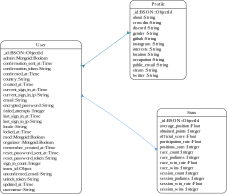
\includegraphics{datamodel1.png}
  \end{center}
  \caption[Modelo de relaciones entre usuario, perfil y estadísticas]{Modelo de relaciones entre usuario, perfil y estadísticas}
  \label{fig:datamodels1}
\end{figure}

\begin{figure}[H]
  \begin{center}
    \includegraphics{datamodel2.png}
  \end{center}
  \caption[Modelo de relación entre temporada, autos y pistas]{Modelo de relación entre temporada, autos y pistas}
  \label{fig:datamodels2}
\end{figure}

\begin{figure}[H]
  \begin{center}
    \includegraphics{datamodel3.png}
  \end{center}
  \caption[Modelo de relaciones entre temporada, ranking y sesiones con sus componentes]{Modelo de relaciones entre temporada, ranking y sesiones con sus componentes}
  \label{fig:datamodels3}
\end{figure}

\begin{figure}[H]
  \begin{center}
    \includegraphics{datamodel4.png}
  \end{center}
  \caption[Modelo de relación entre sesión, carrera y entrada de corredor]{Modelo de relación entre sesión, carrera y entrada de corredor}
  \label{fig:datamodels4}
\end{figure}

\newpage

\section{Esquema de la Base de Datos}
Todas las bases de datos dentro de MongoDB están prefijadas utilizando el término ''rv'' (Re-Volt). Por ejemplo, la base de datos que almacena las colecciones de autos se llama ''rv\_cars'', la de los usuarios ''rv\_users'', etc.

A continuación, se exponen fragmentos de código de Ruby con los modelos definidos para este proyecto. Los fragmentos de código están en formato de \textbf{mongoid} (librería de Ruby para MongoDB). Este formato se compone de la declaración de los campos en los modelos mismos, especificando tipo y otras restricciones asociadas. Además, se mezcla el concepto de relaciones entre modelos de Ruby on Rails.

Para facilitar la comprensión de los esquemas de bases de datos presentados a continuación, se ha confeccionado una tabla que contiene una pequeña especificación de los atributos utilizados para definir los modelos en el formato de mongoid.

\begin{center}
  \begin{tabular}{ | p{6cm} | p{9cm} |}
    \hline
    \multicolumn{1}{|c|}{\textbf{Atributo}} & \multicolumn{1}{|c|}{\textbf{Detalle}} \\
    \hline
    
    {\textbf{store\_in}} & Declara el nombre de la base de datos de mongo en donde los documentos de este modelo serán almacenados.\\ \hline
    {\textbf{field}} & Declara el nombre de un campo del modelo. \\ \hline
    {\textbf{embeds\_many}} & Declara que el modelo contendrá una colección de modelos anidados. \\ \hline
    {\textbf{accepts\_nested\_attributes\_for}} & Declara que el modelo aceptará atributos para los modelos anidados que éste contenga. \\ \hline
    {\textbf{validates\_presence\_of}} & Valida si el campo proveído no está vacío al momento de guardar el modelo en la base de datos. \\ \hline
    {\textbf{belongs\_to}} & Declara que el modelo tendrá una referencia por ID a otro modelo, quedando esta registrada como un atributo.
    \\ \hline
    {\textbf{has\_many}} & Declara que el modelo podrá ser referenciado por ID desde varios otros modelos. \\ \hline
    {\textbf{has\_one}} & Declara que el modelo contará con una referencia singular por ID a otro modelo. \\ \hline
    {\textbf{validates}} & Declara una o más validaciones para un campo del modelo, tales como su presencia garantizada, singularidad, tamaño mínimo o máximo, entre otras.\\ \hline
  \end{tabular}
  
  \captionof{table}{Tabla de especificación de atributos de esquema de la base datos}\label{table:schema}
\end{center}

\begin{listing}
  \begin{minted}[mathescape,
    numbersep=5pt,
    frame=single,
    framesep=2mm]{ruby}
class Season
  include Mongoid::Document
  include Mongoid::Timestamps
  include Mongoid::MultiParameterAttributes
  
  store_in :database => 'rv_seasons'
  
  has_many :rankings
  has_many :cars
  has_many :tracks
  
  embeds_many :racer_result_entries
  
  accepts_nested_attributes_for :racer_result_entries
  
  field :name, :type => String
  field :start_date, :type => Date
  field :end_date, :type => Date
  field :current, :type => Boolean, :default => false
  
  validates_presence_of :name
  validates_presence_of :start_date
  validates_presence_of :current
  
  validates_uniqueness_of :name
end
  \end{minted}
\end{listing}

\begin{listing}
  \begin{minted}[mathescape,
    numbersep=5pt,
    gobble=2,
    frame=single,
    framesep=2mm]{ruby}
  class Ranking
    include Mongoid::Document
    include Mongoid::Timestamps
    
    store_in :database => 'rv_rankings'
    
    belongs_to :season
    has_many :sessions
    
    embeds_many :racer_result_entries
    
    accepts_nested_attributes_for :racer_result_entries
    
    field :number, :type => Integer
    
    validates_presence_of :number
  end
  \end{minted}
\end{listing}

\begin{listing}
  \begin{minted}[mathescape,
    numbersep=5pt,
    gobble=2,
    frame=single,
    framesep=2mm]{ruby}
  class Session
    include Mongoid::Document
    include SessionLogUploader::Attachment(:session_log)
    include Mongoid::Timestamps
    
    store_in :database => 'rv_sessions'
    
    belongs_to :ranking
    embeds_many :races
    embeds_many :racer_result_entries
    
    accepts_nested_attributes_for :racer_result_entries
    
    field :number, :type => Integer
    field :host, :type => String
    field :version, :type => String
    field :physics, :type => String
    field :protocol, :type => String
    field :pickups, :type => Boolean
    field :date, :type => Date
    field :teams, :type => Boolean
    field :category, :type => Integer
    field :session_log_data, :type => String
    
    validates_presence_of :number
    validates_presence_of :host
    validates_presence_of :version
    validates_presence_of :physics
    validates_presence_of :protocol
    validates_presence_of :date
    validates_presence_of :session_log
    validates_presence_of :teams
    validates_presence_of :category
  end
  \end{minted}
\end{listing}

\begin{listing}
  \begin{minted}[mathescape,
    numbersep=5pt,
    gobble=2,
    frame=single,
    framesep=2mm]{ruby}
  class User
    include Mongoid::Document
    include Mongoid::Timestamps
    
    store_in :database => 'rv_users'
    
    USERNAME_REGEX = /\A([A-Z0-9_]{1,16}|[0-9a-f]{24})\z/
    
    validates :email, :presence => true, :uniqueness => true
    validates :username, :presence => true, 
    :uniqueness => true, 
    :length => { :minimum => 2, :maximum => 16 }
    validates_format_of :username, :with => USERNAME_REGEX
    
    belongs_to :team, :optional => true
    has_one :team
    
    embeds_one :profile
    embeds_one :stats
    accepts_nested_attributes_for(
    :profile,
    :update_only => true,
    :allow_destroy => false
    )
    accepts_nested_attributes_for(:stats,
    :update_only => true,
    :allow_destroy => false
    )
    
    before_create :create_profile
    before_create :create_stats
    
    field :admin, :type => Boolean, :default => false
    field :mod, :type => Boolean, :default => false
    field :organizer, :type => Boolean, :default => false
    field :locale, :type => String, :default => 'en_us'
    field :country, :type => String
  end
  \end{minted}
\end{listing}

\begin{listing}
  \begin{minted}[mathescape,
    numbersep=5pt,
    gobble=2,
    frame=single,
    framesep=2mm]{ruby}
  class Race
    include Mongoid::Document
    include Mongoid::Attributes::Dynamic
    
    embedded_in :session
    
    embeds_many :racer_entries
    
    field :track_name, :type => String
    field :laps, :type => Integer
    field :racers_count, :type => Integer
    
    validates_presence_of :track_name
    validates_presence_of :laps
    validates_presence_of :racers_count
  end
  \end{minted}
\end{listing}

\begin{listing}
  \begin{minted}[mathescape,
    numbersep=5pt,
    gobble=2,
    frame=single,
    framesep=2mm]{ruby}
  class RacerEntry
    include Mongoid::Document
    include Mongoid::Attributes::Dynamic
    
    embedded_in :race
    
    field :car_name, :type => String
    field :position, :type => Integer
    field :username, :type => String
    field :time, :type => String
    field :best_lap, :type => String
    field :finished, :type => Mongoid::Boolean
    field :cheating, :type => Mongoid::Boolean
    
    validates_presence_of :car_name
    validates_presence_of :position
    validates_presence_of :username
    validates_presence_of :time
    validates_presence_of :best_lap
    validates_presence_of :finished
    validates_presence_of :cheating
  end
  \end{minted}
\end{listing}

\begin{listing}
  \begin{minted}[mathescape,
    numbersep=5pt,
    gobble=2,
    frame=single,
    framesep=2mm]{ruby}
  class Profile
    include Mongoid::Document
    
    embedded_in :user
    
    field :about, :type => String
    field :gender, :type => String
    field :public_email, :type => String
    field :location, :type => String
    field :discord, :type => String
    field :github, :type => String
    field :instagram, :type => String
    field :crowdin, :type => String
    field :steam, :type => String
    field :twitter, :type => String
    field :occupation, :type => String
    field :interests, :type => String
  end
  \end{minted}
\end{listing}

\begin{listing}
  \begin{minted}[mathescape,
    numbersep=5pt,
    gobble=2,
    frame=single,
    framesep=2mm]{ruby}
  class Stats
    include Mongoid::Document
    
    embedded_in :user
    
    field :race_wins, :type => Integer
    field :race_win_rate, :type => Float
    field :race_podiums, :type => Integer
    field :race_count, :type => Integer
    field :positions_sum, :type => Integer
    field :session_wins, :type => Integer
    field :session_win_rate, :type => Float
    field :session_podiums, :type => Integer
    field :session_count, :type => Integer
    field :average_position, :type => Float
    field :participation_rate, :type => Float
    field :official_score, :type => Float
    field :obtained_points, :type => Integer
  end
  \end{minted}
\end{listing}

\begin{listing}
  \begin{minted}[mathescape,
    numbersep=5pt,
    gobble=2,
    frame=single,
    framesep=2mm]{ruby}
  class Car
    include Mongoid::Document
    include Mongoid::Timestamps
    
    store_in :database => 'rv_cars'
    
    belongs_to :season
    
    field :name, :type => String
    field :speed, :type => Float
    field :accel, :type => Float
    field :weight, :type => Float
    field :multiplier, :type => Float
    field :folder_name, :type => String
    field :category, :type => Integer
    field :stock, :type => Boolean, :default => false
    
    validates_presence_of :name
    validates_presence_of :speed
    validates_presence_of :accel
    validates_presence_of :weight
    validates_presence_of :multiplier
    validates_presence_of :folder_name
    validates_presence_of :category
    validates_presence_of :stock
  end
  \end{minted}
\end{listing}

\begin{listing}
  \begin{minted}[mathescape,
    numbersep=5pt,
    gobble=2,
    frame=single,
    framesep=2mm]{ruby}
  class Track
    include Mongoid::Document
    include Mongoid::Timestamps
    
    store_in :database => 'rv_tracks'
    
    belongs_to :season
    
    field :name, :type => String
    field :short_name, :type => String
    field :difficulty, :type => Integer
    field :length, :type => Integer
    field :folder_name, :type => String
    field :stock, :type => Boolean, :default => false
    
    validates_presence_of :name
    validates_presence_of :short_name
    validates_presence_of :difficulty
    validates_presence_of :length
    validates_presence_of :folder_name
    validates_presence_of :stock
  end
  \end{minted}
\end{listing}

\begin{listing}
  \begin{minted}[mathescape,
    numbersep=5pt,
    gobble=2,
    frame=single,
    framesep=2mm]{ruby}
  class RacerResultEntry
    include Mongoid::Document
    
    embedded_in :season
    embedded_in :ranking
    embedded_in :session
    
    field :username, :type => String
    field :country, :type => String
    field :session_count, :type => Integer
    field :race_count, :type => Integer
    field :positions_sum, :type => Integer
    field :average_position, :type => Float
    field :obtained_points, :type => Integer
    field :official_score, :type => Float
    field :participation_multiplier, :type => Float
    field :team, :type => String
    
    validates_presence_of :username
    validates_presence_of :country
  end
  \end{minted}
\end{listing}

\clearpage

\section{Diseño de Interfaz}
El diseño de las interfaces de Re-Volt America ha sido debidamente cuidado al ser implementado en aplicación desarrollada.

En primer lugar, contamos con una página de inicio con el título de la comunidad de Re-Volt America, junto con varias imágenes del juego para que este pueda ser inmediatamente reconocido por quien visite el portal.

En la parte superior, se encuentra la barra de navegación principal, la cual incluye, de izquierda a derecha:
\begin{itemize}
  \item El logo de RVA.
  \item Botones para acceder a las secciones más importantes de la web.
  \item Un botón para poder registrarse, iniciar sesión o visualizar información del perfil en caso de existir una sesión iniciada.
\end{itemize}

\begin{figure}[H]
  \begin{center}
    \includegraphics[width=15cm, height=8cm]{img/landing.png} 
  \end{center}
  \caption[Landing page de RVA]{Landing page de RVA}
  \label{fig:landing}
\end{figure}

Dentro de las secciones de autos, pistas y sesiones se cuenta con una barra de sub-navegación, la cual integra todos los elementos de una temporada, dando acceso al usuario de manera más práctica a toda la información que este podría necesitar.

\begin{figure}[H]
  \begin{center}
    \includegraphics[width=15cm, height=8cm]{img/landing.png} 
  \end{center}
  \caption[Página de autos de RVA]{Página de autos de RVA}
  \label{fig:cars}
\end{figure}

\begin{figure}[H]
  \begin{center}
    \includegraphics[width=15cm, height=8cm]{img/tracks.png} 
  \end{center}
  \caption[Página de pistas de RVA]{Página de pistas de RVA}
  \label{fig:tracks}
\end{figure}

El diseño de la interfaz de las sesiones respeta fielmente el formato original de RVA.

\begin{figure}[H]
  \begin{center}
    \includegraphics[width=15cm, height=8cm]{img/tracks.png} 
  \end{center}
  \caption[Página de sesión de RVA]{Página de sesión de RVA}
  \label{fig:session}
\end{figure}

La el diseño de la página de perfil de los usuarios cuenta con su nombre en grande, un resumen de sus estadísticas, posición en el ranking y un pequeño historial de las últimas sesiones en las que han participado.

\begin{figure}[H]
  \begin{center}
    \includegraphics[width=15cm, height=8cm]{img/profile1.png} 
  \end{center}
  \caption[Página de perfil de usuario de RVA]{Página de perfil de usuario de RVA}
  \label{fig:profile}
\end{figure}

Por último, la página de estadísticas sigue un formato simple de tabla de resultados, con un selector que permite filtrar dichos resultados según diversos criterios.

\begin{figure}[H]
  \begin{center}
    \includegraphics[width=15cm, height=8cm]{img/stats.png} 
  \end{center}
  \caption[Página de estadísticas globales de RVA]{Página de estadísticas globales de RVA}
  \label{fig:stats}
\end{figure}

\subsection{Paleta de Colores y Tipografía}
Como preámbulo principal en cuanto a la pelta de colores y tipografía de RVA, debemos recordar que esta comunidad nace de un grupo de jugadores de Re-Volt, no de una empresa o compañía con estándares definidos. Por lo tanto, para comprender los orígenes de estos elementos, debemos remontarnos a los inicios de Re-Volt America por el año 2017.

Durante los inicios de RVA, se diseña su logo principal, el cual puede apreciarse en la \autoref{fig:rva-logo}.

\begin{figure}[H]
  \begin{center}
    \includegraphics[width=8cm, height=8cm]{img/rva.png} 
  \end{center}
  \caption[Logotipo de RVA]{Logotipo de RVA}
  \label{fig:rva-logo}
\end{figure}

Del logo de RVA, se derivan los colores blanco y negro (absolutos), los cuales son utilizados como paleta principal para la comunidad.

Así como los colores, la comunidad ha utilizado una fuente muy similar a la empleada en el logotipo a lo largo de los años. Esta fuente se titula ''Nissan Opti'', desarrollada originalmente por Castcraft Software. La caracterización de esta compañía tipográfica puede verse a continuación en la \autoref{fig:optifont}.

\begin{figure}[H]
  \begin{center}
    \includegraphics{img/optifont.png} 
  \end{center}
  \caption[Arte de Castcraft Software]{Arte de Castcraft Software}
  \label{fig:optifont}
\end{figure}

De la misma forma, nacen las paletas de colores para las tablas de resultados de sesiones y rankings acumulados. Estas últimas pueden apreciarse a continuación.


\begin{figure}[H]
  \begin{center}
    \includegraphics[width=16cm, height=8cm]{img/session_table.png} 
  \end{center}
  \caption[Tabla de resultados de sesión de RVA]{Tabla de resultados de sesión de RVA}
  \label{fig:session-table}
\end{figure}

\begin{figure}[H]
  \begin{center}
    \includegraphics[width=16cm, height=9cm]{img/ranking_table.png} 
  \end{center}
  \caption[Tabla de ranking de RVA]{Tabla de ranking de RVA}
  \label{fig:ranking-table.png}
\end{figure}

La paleta de colores de las tablas de resultados, junto a su definición en RGB (Red, Green, Blue), puede encontrarse en la \autoref{fig:rva-session-colors} a continuación.

\begin{figure}[H]
  \begin{center}
    \includegraphics[width=15cm, height=10cm]{img/rva_session_colors.png} 
  \end{center}
  \caption[Paleta de colores de sesiones de RVA]{Paleta de colores de sesiones de RVA}
  \label{fig:rva-session-colors}
\end{figure}

\newpage

\section{Diseño de Arquitectura}
El proyecto, en su estado actual, hace uso de un servidor propio, el cual contiene los servicios web, bases de datos y caché. Todo en una sola máquina. Independientemente de donde se termine alojando, la aplicación web estará disponible en ''https://rva.lat/''.

Además de esto, la planificación contempla dos servicios externos, que actualmente son proveídos por GitHub pages, los cuales sirven como repositorios de almacenamiento de datos masivos. Dichos repositorios se encargan actualmente de servir información y assets como las imágenes de las pistas y autos que la web ofrece a los usuarios:

\begin{itemize}
  \item https://tracks.rva.lat/: Repositorio de pistas de RVA.
  \item https://cars.rva.lat/: Repositorio de autos de RVA.
\end{itemize}

A continuación, se muestra un diagrama que ilustra todo el proceso de interacción entre servicios y usuarios:

\begin{figure}[H]
  \begin{center}
    \includegraphics[width=16cm, height=11cm]{img/architecture.png} 
  \end{center}
  \caption[Diagrama de arquitectura de RVA]{Diagrama de arquitectura de RVA}
  \label{fig:architecture.png}
\end{figure}

Tal como se puede apreciar en la ilustración anterior, la arquitectura que da soporte a la aplicación web de RVA se concentra en un servidor, con dos almacenes de datos. Podemos ver que los usuarios juegan la sesión, el host de la sesión sube el Session Log a la web, y los usuarios pueden visitar la misma web para revisar los resultados

\newpage

\section{Estructura del Código}
El proyecto, al ser una aplicación hecha en el framework de Ruby on Rails, sigue el patrón de MVC (Model View Controller) o modelo, vista, controlador. El árbol de directorios del proyecto se ve de la siguiente manera.

\begin{figure}[H]
  \begin{center}
    \includegraphics[height=16cm]{img/tree.png} 
  \end{center}
  \caption[Árbol de directorios del proyecto]{Árbol de directorios del proyecto}
  \label{fig:tree.png}
\end{figure}

Dentro los archivos relevantes para la estructura del código, tenemos aquellos archivos en los que se definen dependencias y módulos de despliegue.

\begin{center}
  \begin{tabular}{ | l | p{12.5cm} |}
    \hline
    \multicolumn{1}{|c|}{\textbf{Archivo}} & \multicolumn{1}{|c|}{\textbf{Detalle}} \\
    \hline
    
    {\textbf{Capfile}} & Contiene la carga de módulos para el despliegue de la aplicación. \\ \hline
    {\textbf{Gemfile}} & Contiene todas las dependencias del proyecto, con sus respectivas versiones. \\ \hline
  \end{tabular}
  
  \captionof{table}{Tabla archivos de dependencias y módulos de despliegue}\label{table:dependencies}
\end{center}

\subsection{Estándres de Codificación}
El código de este proyecto sigue las recomendaciones estándar para la programación con Ruby, y otros estándares de manera consistente:
\begin{itemize}
  \item Toda la base de código y documentación debe estar escrita en inglés.
  \item Eng eneral, todo el proyecto sigue las convenciones de nombrado y otros lineamientos útiles del sitio de RubyStyle.
  \item Se utilizan linebreaks (EOL - End of Line) CRLF.
  \item Se utilizan dos espacios para la indentación del código, no tabulaciones.
  \item La codificación del proyecto es en UTF-8. 
\end{itemize}

\subsection{Caché con Redis}
Las llaves o entradas del caché de Redis son nombradas en minúscula, y los espacios que pudieran existir en ellas son reemplazados por guiones bajos. En caso de llaves compuestas, se utiliza el siguiente formato:

\begin{itemize}
  \item \text{object\_type:id}
  \item \text{object\_type:id\#field}
  \item \text{object\_type:id\#embedded\_object:id}
  \item \text{object\_type:id\#embedded\_object:id\#field}
\end{itemize}

\begin{longlisting}
  \begin{minted}[mathescape,
    linenos,
    numbersep=5pt,
    breaklines,
    frame=single,
    framesep=2mm]{ruby}  
def show
  require 'rva_calculate_results_service'
	
  @count = 0
  @rva_results = Rails.cache.fetch("Session:#{@session.id}") do
    RvaCalculateResultsService.new(@session).call
  end
	
  respond_with @session do |format|
    format.json { render :layout => false }
  end  
end
  \end{minted}
\end{longlisting}


\subsection{Backend}

\begin{center}
  \begin{tabular}{ | l | p{12.5cm} |}
    \hline
    \multicolumn{1}{|c|}{\textbf{Directorio}} & \multicolumn{1}{|c|}{\textbf{Detalle}} \\
    \hline
    
    {\textbf{controllers}} & Contiene todos los controladores de Rails, los cuales manejan todas las peticiones web del usuario. \\ \hline
    
    {\textbf{helpers}} & Contiene todas las clases utilitarias, las cuales pueden ser utilizadas para asistir a las clases de modelos, vistas y controladores. \\ \hline
    
    {\textbf{javascript}} & Todo el código de JavaScript utilizado por la aplicación a nivel web se almacena en este directorio.\\ \hline
    
    {\textbf{models}} & Contiene todas las clases que modelan y envuelven los datos almacenados en la base de datos de la aplicación. \\ \hline
    
    {\textbf{services}} & Contiene todas las clases de servicio de la aplicación. Las clases de servicio son aquellos procesos complejos compuestos de mucho código, los cuales se abstraen en servicios para no polucionar los controladores que los requieren. \\ \hline
    
    {\textbf{uploaders}} & Contiene todas las clases relacionadas con la subida de archivos. \\ \hline
    
    {\textbf{config}} & Contiene toda la configuración de la aplicación, como las rutas, inicializadores de librerías, configuración de despliegue, declaración de los entornos de Rails (development, production), configuración de la base de datos y archivos de idioma para la localización del proyecto.\\ \hline
  \end{tabular}
  
  \captionof{table}{Tabla de directorios del backend del proyecto}\label{table:backend}
\end{center}

\subsection{Frontend}

\begin{center}
  \begin{tabular}{ | l | p{12.5cm} |}
    \hline
    \multicolumn{1}{|c|}{\textbf{Directorio}} & \multicolumn{1}{|c|}{\textbf{Detalle}} \\
    \hline
    
    {\textbf{views}} & Contiene todas las vistas de la aplicación. Todo lo que el usuario ve en la aplicación web tiene su archivo de vista que lo representa. \\ \hline
    
    {\textbf{assets}} & Todas las imágenes, hojas de estilo y demás artefactos requeridos por la aplicación para su correcto funcionamiento y diseño. \\ \hline
    
    {\textbf{public}} & Todos los archivos estáticos servidos por la página pueden encontrarse aquí. Cosas como las páginas de error (404, 422, 500, etc.), estilos compilados, entre otros.\\ \hline
  \end{tabular}
  
  \captionof{table}{Tabla de directorios del frontend del proyecto}\label{table:frontend}
\end{center}


% Training
\chapter{Plan de Capacitación, Implantación y Puesta en Marcha}

\subsection{Estado del Proyecto}
Actualmente, el proyecto se encuentra finalizado.

EXPLICAR TODO LO QUE SE TERMINÓ

Además de lo anterior, se ha programado e implementado completamente la lógica operativa interna de Re-Volt America dentro del sistema, por lo que este puede recibir archivos Session Log, procesarlos y almacenarlos correctamente, mostrando al usuario una vista interpretada de los resultados de la sesión.

\subsection{Proyecciones del Proyecto}



% Conclusión
\chapter{Conclusión del Proyecto}
Para finalizar este informe, a continuación se plantean una serie de conclusiones a las que se llegó luego de llevar a cabo el desarrollo e implementación del software:

\begin{itemize}
	\item En relación con elaborar una propuesta que consiguiera atender las necesidades y problemas de los usuarios de Re-Volt America, con respecto al almacenamiento y visualización de resultados de partidas online, podemos decir que se logró cumplir dicho objetivo gracias al software desarrollado.
	\item De acuerdo con el objetivo que hablaba de diseñar una solución de software de procesamiento de datos de sesiones multijugador oficiales de las sesiones de carreras en línea, además de estadísticas personales, podemos decir que es un objetivo que fue cumplido completamente ya que, tanto el procesamiento de datos como las estadísticas por usuario fueron exitosamente implementadas.
	\item En relación con el objetivo de implementar una aplicación web que permitiera a los organizadores de sesiones de carreras en línea subir y publica los resultados de dichas carreras podemos decir que, en conclusión, dicho objetivo fue cumplido con éxito, ya que el software, incluso en su estado actual, ya puede realizar la importación de Session Logs, el cálculo y procesamiento de resultados en el formato de RVA, y finalmente mostrar dichos resultados por pantalla a quien los solicite desde la web.
	\item El proyecto ha permitido demostrar las competencias que se esperan de un ingeniero de ejecución en computación e informática, ya que se han aplicado la identificación de necesidades, análisis y el diseño de soluciones informáticas para Re-Volt America, logrando desarrollar una solución que le permite a la comunidad tener un mejor manejo de sus procesos internos, registros de datos más fiables y una experiencia de usuario mejorada en comparación con su sistema original. 
	\item El proyecto ha sido realmente enriquecedor desde el punto de vista del desarrollo de software puesto que, dentro del área en que fue realizado, fue posible aplicar diversas tecnologías, técnicas de diseño de software, despliegue de aplicaciones e implementación de estándares de calidad, todo en un mismo contexto que cierra de manera redonda el ciclo de desarrollo que se espera pueda ser alcanzado por un ingeniero de software.
\end{itemize}


% Anexos
\chapter{Anexos}

\section{Anexos de Pruebas de Aceptación}

\section{Anexos de Recopilación de Información}
REUNIONES Y RECOLECCION DE INFORMACION DE USO ETC

\section{Anexo Diccionario de Datos}

\section{Anexo Aspectos de Gestión de Proyectos}

\subsection{Anexo Carta Gantt}

\includegraphics{gantt.png}

\subsection{Riesgos de Alto Nivel, Impacto y Estrategia}

\subsection{Anexo Estimación Casos de Uso}

\subsection{Anexo Resumen de Esfuerzo}

\section{Anexos Retrospectiva del Proyecto}

\subsection{Anexo Iteraciones en el Desarrollo}

COMMITS RELEVANTES HITOS DE DESARROLLO QUE MOSTRÉ A MIS USUARIOS

\end{document}




















